\documentclass[12pt,a4paper]{article}
\usepackage[utf8]{inputenc}
\usepackage[english]{babel}
\usepackage{amsmath, amssymb, amsthm}
\usepackage{siunitx}
\usepackage{graphicx}
\usepackage{booktabs}
\usepackage{float}
\usepackage[margin=2.5cm]{geometry}
\usepackage{hyperref}
\usepackage[natbibapa]{apacite}

\title{Beyond Porosity: A Bayesian Model-Comparison Framework for Biomass Retention in Anaerobic Packed Beds Using Hydraulic Signatures}
\author{Moses I. A. Mosia \and [Co-Authors]}
\date{\today}

\begin{document}

\maketitle

\begin{abstract}
Conventional wisdom in anaerobic reactor design assumes that packing materials with higher porosity provide better biomass retention by increasing interstitial capacity and reducing clogging. However, experimental data from this study contradict this ``Volumetric Assumption'': spherical glass marbles (porosity 0.40) retained only 19.1~g of sludge, while irregular pea gravel (porosity 0.36) retained 126.9~g---a $6.7\times$ difference demonstrating that the system is ``friction-limited'' rather than ``volume-limited.'' This paper develops a Bayesian model-comparison framework to test whether porosity alone explains retention, or whether morphology-sensitive ``hydraulic signatures'' extracted from pressure-drop data provide superior predictive power. A two-stage hierarchical approach was employed: Stage~I calibrated medium-specific permeability ($k$) and Forchheimer inertial coefficients ($\beta$) via Bayesian Darcy--Forchheimer regression; Stage~II compared four competing Beta-regression retention models (volumetric, hydraulic, combined, and geometry-derived) using Pareto-smoothed importance sampling leave-one-out cross-validation (PSIS-LOO). Results show that the combined model incorporating both porosity and hydraulic signatures achieved the highest expected log predictive density (ELPD$_{\mathrm{LOO}}=-0.995$) and pseudo-BMA weight (0.40), while the porosity-only model systematically over-predicted retention for smooth media. Posterior sign probabilities strongly favored positive effects for both permeability ($P(b_{\log k}>0)=0.88$) and Forchheimer coefficient ($P(b_{\log(1+\beta)}>0)=0.95$), supporting a friction-limited retention mechanism. These findings suggest that underdrain system design should prioritize frictional damping characteristics over simple hydraulic conductivity, with packing material selection guided by posterior ranking probabilities rather than deterministic porosity-based criteria.
\end{abstract}

\section{Introduction}

\subsection{The Research Problem}
Packed-bed anaerobic reactors are routinely designed with a volumetric heuristic in which higher void fraction is assumed to imply improved biomass retention through increased interstitial capacity and delayed clogging. However, the packing-media outcomes in the present study exhibit a counter-ordering that contradicts this ``Volumetric Assumption'': spherical glass marbles with moderate porosity ($\varepsilon=0.40$) retained only 19.1~g of sludge, while irregular pea gravel with lower porosity ($\varepsilon=0.36$) retained 126.9~g. This paradox suggests that the system is ``friction-limited'' rather than ``volume-limited,'' and that current models treating packing material merely as passive void space ignore the critical role of packing morphology---specifically roughness and sphericity---in mechanically dampening hydrodynamic forces that would otherwise displace retained biomass.

This paper develops a Bayesian, uncertainty-aware evidence framework that tests whether retention is adequately explained by porosity alone, or whether packing morphology must be represented through measurable ``hydraulic signatures'' extracted from pressure-drop data. The central research questions are: (i)~whether a porosity-only model can predict observed retention fractions once measurement uncertainty is propagated; (ii)~whether morphology-sensitive descriptors improve out-of-sample predictive performance under principled Bayesian model comparison; and (iii)~whether an engineering-facing probabilistic ranking of media resilience can be derived as a posterior quantity suitable for design decisions.

\subsection{Research Questions}
This study addresses the following key questions through Bayesian inference and model comparison:
\begin{enumerate}
    \item Why does higher porosity correlate with lower sludge retention in smooth media, defying volumetric logic, and can this counter-ordering be reproduced within posterior uncertainty by any single-predictor model?
    \item Do hydraulic signatures---permeability ($k$) and inertial resistance coefficient ($\beta$)---extracted from pressure-drop data provide stronger statistical evidence for explaining between-media retention differences than porosity alone?
    \item Can a probabilistic ranking of packing media for retention resilience be derived from posterior distributions, enabling uncertainty-aware design decisions rather than deterministic index-based selection?
\end{enumerate}

\subsection{Objectives}
The primary objectives of this research are:
\begin{enumerate}
    \item To experimentally falsify the ``Volumetric Assumption'' using Bayesian model comparison (PSIS-LOO cross-validation) across competing retention hypotheses applied to five packing media (glass marbles, pea gravels, white pebbles, small pumice stones, and medium pumice stones).
    \item To develop a two-stage Bayesian hierarchical framework that separates hydraulic signature estimation (Stage~I: Darcy--Forchheimer calibration) from retention prediction (Stage~II: Beta regression), thereby propagating uncertainty without circularity.
    \item To propose a new design criterion for underdrain systems that prioritizes frictional damping characteristics over simple hydraulic conductivity, supported by posterior ranking probabilities rather than ad hoc deterministic indices.
\end{enumerate}

\section{Materials and methods}

\subsection{Data sources and scope}
All analyses were performed on the archived experimental workbook \texttt{DEng data.xlsx}, using two sheets as primary data sources for Paper~2. The \texttt{Packing materials} sheet reports packed-bed geometry, void volumes, porosities, and end-point sludge retention outcomes for five packing media. The \texttt{Underdrain system} sheet reports, for each medium, material descriptors (including sphericity and characteristic diameter) and pressure-drop measurements across a controlled range of superficial liquid velocities in water at \SI{35}{\celsius}. The methodological objective is comparative and inferential: the study does not attempt to reconstruct micro-scale multiphase hydrodynamics, but rather to determine whether geometry-sensitive descriptors provide stronger statistical evidence for explaining between-media retention differences than porosity alone, while propagating uncertainty in both descriptor estimation and outcome measurement.

\subsection{Packed-bed retention module and retention outcomes}
The packed-bed module used for sludge retention accounting has internal diameter $D=\SI{0.086}{m}$ and packed height $H=\SI{0.05}{m}$ as recorded in the \texttt{Packing materials} sheet. The geometric bed volume is therefore
\begin{equation}
V_{\mathrm{bed}}=\frac{\pi D^2}{4}H,
\end{equation}
which is consistent with the recorded packed-bed total volume of \SI{290}{mL} for all media in the retention dataset. For each packing medium $j$, the dataset provides the measured void volume $V_{\mathrm{void},j}$ and the corresponding porosity
\begin{equation}
\phi_j=\frac{V_{\mathrm{void},j}}{V_{\mathrm{bed}}}.
\end{equation}
The dataset further provides the initial sludge mass loaded $M_{0,j}$, the washed-out sludge mass $M_{\mathrm{out},j}$, and the retained sludge mass $M_{\mathrm{ret},j}$ at the end of the test horizon. These satisfy the mass-balance identity $M_{\mathrm{ret},j}=M_{0,j}-M_{\mathrm{out},j}$; the recorded values were used as given, and consistency checks were applied to identify transcription errors.

The primary response variable for Bayesian modelling is the retention fraction
\begin{equation}
R_j=\frac{M_{\mathrm{ret},j}}{M_{0,j}}, \qquad R_j\in(0,1),
\end{equation}
which corresponds to the recorded ``sludge retention capacity.'' A secondary response variable is a void-normalized retained mass density
\begin{equation}
\tilde{M}_j=\frac{M_{\mathrm{ret},j}}{V_{\mathrm{void},j}},
\end{equation}
which is used diagnostically to evaluate whether a medium with larger void volume simply retains more biomass because more space is available, or whether the retention efficiency per unit void volume differs systematically across media.

\subsection{Underdrain hydrodynamic characterization and hydraulic signatures}
The \texttt{Underdrain system} sheet provides pressure-drop measurements $\Delta P_{j}(v)$ for each medium $j$ over a set of superficial velocities $v$ in the approximate range $4\times 10^{-6}$ to $4\times 10^{-5}\,\si{m\,s^{-1}}$. Water properties at \SI{35}{\celsius} are recorded as density $\rho=\SI{993.95}{kg\,m^{-3}}$ and dynamic viscosity $\mu=\SI{7.255e-4}{Pa\,s}$. The bed height for the pressure-drop column is recorded as $L=\SI{0.09}{m}$; this column is treated as a characterization apparatus for extracting bed-scale resistance descriptors rather than as a geometrically identical replica of the \SI{0.05}{m} retention module.

A laminar-flow check was performed using the particle Reynolds number based on a representative particle diameter $d_{p,j}$ provided in the same sheet:
\begin{equation}
\mathrm{Re}_{p,j}(v)=\frac{\rho v d_{p,j}}{\mu}.
\end{equation}
Given the velocity range and diameters in the dataset, $\mathrm{Re}_{p,j}(v)\ll 1$ holds across all media, supporting a creeping-to-laminar regime in which inertia is weak and pressure drop is expected to be approximately linear in $v$.

Hydraulic ``signatures'' were extracted from the $\Delta P$--$v$ relationship using two nested resistance models. The first is Darcy flow through a homogeneous porous medium,
\begin{equation}
\Delta P_{j}(v)=\frac{\mu L}{k_j}v + \epsilon_{j}(v),
\end{equation}
where $k_j$ is an effective permeability and $\epsilon_j(v)$ represents measurement error and structural deviations from linearity. The second is a Darcy--Forchheimer extension,
\begin{equation}
\Delta P_{j}(v)=\frac{\mu L}{k_j}v + \rho L\,\beta_j v^2 + \epsilon_{j}(v),
\end{equation}
where $\beta_j$ is an inertial resistance coefficient. In a strictly creeping-flow regime, the posterior for $\beta_j$ is expected to concentrate near zero; nevertheless, this term is retained as a robustness check against minor inertial contributions or systematic curvature in the recorded $\Delta P$ values. The inferred $(k_j,\beta_j)$ pairs constitute media-specific hydraulic signatures that are estimable from the archived dataset and usable as morphology-sensitive predictors in the retention model without requiring direct roughness measurements.

\subsection{Geometry descriptors and uncertainty representation}
The packed-media comparison requires a representation of ``geometry'' that is distinct from porosity. In this study, geometry is represented in two complementary ways. First, the hydraulic signature $(k_j,\beta_j)$ is treated as an empirical descriptor of pore-scale structure, tortuosity, and flow-path complexity, acknowledging that it is not a unique mapping from shape to mechanics but is nevertheless a reproducible medium-level measure derived from the pressure-drop experiments. Second, the \texttt{Underdrain system} sheet reports a sphericity value $\Psi_j$ for some media; when available, this value is used as an additional morphology proxy through the irregularity index
\begin{equation}
H_{\mathrm{geo},j} = 1-\Psi_j,
\end{equation}
which is interpreted as an entropy-like irregularity score (monotone in deviation from a sphere) rather than as a thermodynamic entropy. When $\Psi_j$ is not directly recorded for a medium, $\Psi_j$ is treated as a latent parameter with a prior distribution reflecting a plausible range for the medium's qualitative shape class, so that uncertainty in morphology classification is propagated into retention inferences rather than fixed deterministically.

\subsection{Bayesian modelling framework}
The Bayesian analysis is structured as a two-stage hierarchical model that separates (i) estimation of hydraulic signatures from pressure-drop data and (ii) explanation and prediction of retention outcomes using competing covariate sets. This separation prevents circularity, because retention outcomes do not inform the estimation of $(k_j,\beta_j)$, while uncertainty in the hydraulic signatures is propagated forward into the retention model.

\subsubsection{Stage I: Bayesian calibration of hydraulic signatures}
For each medium $j$ and each observed velocity $v_{i}$ with measured pressure drop $\Delta P_{ij}$, the likelihood is specified as
\begin{equation}
\Delta P_{ij} \sim \mathcal{N}\!\left(\frac{\mu L}{k_j}v_i + \rho L\,\beta_j v_i^2,\;\sigma_{\Delta P,j}^2\right),
\end{equation}
with a medium-specific measurement scale $\sigma_{\Delta P,j}$. Weakly informative priors enforce physical constraints and stabilize inference:
\begin{align}
\log k_j &\sim \mathcal{N}(m_k, s_k^2), \qquad m_k \sim \mathcal{N}(\log 10^{-9}, 2^2), \qquad s_k \sim \mathrm{HalfNormal}(1), \\
\beta_j &\sim \mathcal{N}(0, 1^2)\,\mathbb{I}(\beta_j\ge 0), \\
\sigma_{\Delta P,j} &\sim \mathrm{HalfNormal}(\tau_{\Delta P}),
\end{align}
where the permeability prior is intentionally wide on the log scale and the inertial term is constrained non-negative. The posterior distribution $p(k_j,\beta_j,\sigma_{\Delta P,j}\mid \{\Delta P_{ij}\})$ is summarized by posterior means and credible intervals, and is retained in full for propagation into Stage~II via posterior draws.

\subsubsection{Stage II: Bayesian retention models and hypothesis discrimination}
Retention fractions $R_j$ are modelled with a Beta likelihood to respect the $(0,1)$ support while allowing flexible dispersion:
\begin{equation}
R_j \sim \mathrm{Beta}\!\left(\kappa\,\mu_j,\; \kappa\,(1-\mu_j)\right),
\end{equation}
where $\mu_j\in(0,1)$ is the mean retention for medium $j$ and $\kappa>0$ controls dispersion. Competing hypotheses about retention mechanisms are encoded through alternative predictors for $\mu_j$ using a logit link.

The volumetric model (the ``porosity-only'' hypothesis) is
\begin{equation}
\mathrm{logit}(\mu_j)=a_0 + a_\phi\,\mathrm{logit}(\phi_j).
\end{equation}
The morphology model based on hydraulic signatures is
\begin{equation}
\mathrm{logit}(\mu_j)=b_0 + b_k\,\log k_j + b_\beta\,\log(1+\beta_j),
\end{equation}
where $(k_j,\beta_j)$ are treated as uncertain inputs via posterior draws from Stage~I. A combined model is also fit to assess whether porosity retains explanatory value once hydraulic signatures are included:
\begin{equation}
\mathrm{logit}(\mu_j)=c_0 + c_\phi\,\mathrm{logit}(\phi_j) + c_k\,\log k_j + c_\beta\,\log(1+\beta_j).
\end{equation}
When recorded or inferred sphericity is available, an auxiliary morphology model is considered:
\begin{equation}
\mathrm{logit}(\mu_j)=d_0 + d_H\,H_{\mathrm{geo},j},
\end{equation}
with $\Psi_j$ modelled as latent when not directly observed, thereby avoiding deterministic assignment.

Regularizing priors were used for all regression coefficients to avoid overfitting in the small-$J$ regime:
\begin{equation}
a_0,b_0,c_0,d_0 \sim \mathcal{N}(0,1.5^2), \qquad a_\phi,b_k,b_\beta,c_\phi,c_k,c_\beta,d_H \sim \mathcal{N}(0,1^2),
\end{equation}
and dispersion is assigned
\begin{equation}
\kappa \sim \mathrm{HalfNormal}(5).
\end{equation}
Posterior predictive distributions for $R_j$ were computed for each model and used for both descriptive checking and model comparison.

\subsection{Bayesian model comparison and falsification logic}
The falsification objective is framed as a comparison of predictive adequacy: if porosity is sufficient to explain retention, the porosity-only model should exhibit competitive out-of-sample predictive performance and should reproduce the observed ordering of $R_j$ across media within posterior uncertainty. Predictive model comparison is performed using Pareto-smoothed importance sampling leave-one-out cross-validation (PSIS-LOO) applied to the pointwise log-likelihood, yielding an expected log predictive density (ELPD) for each candidate model. Differences in ELPD are reported with standard errors to quantify evidence strength. Posterior predictive checks complement LOO by evaluating whether the models reproduce (i) the marginal distribution of $R_j$, (ii) the empirical ranking of media, and (iii) the magnitude of the porosity--retention counter-ordering that motivates the study.

Because the number of media is small, model comparison is not treated as a mechanical winner-take-all procedure. Instead, results are interpreted through three aligned criteria: predictive evidence (ELPD), posterior effect sizes and signs for key coefficients, and robustness under sensitivity analyses. This approach supports an evidence-based conclusion of the form that porosity-only explanations are insufficient under the present conditions, and that morphology-sensitive descriptors provide measurable additional explanatory power, while avoiding overconfident mechanistic claims that cannot be uniquely identified from the archived measurements.

\subsection{Derived design metric as a posterior quantity}
An engineering-facing resilience score is defined as a derived quantity, constructed so that uncertainty in its components is propagated through the posterior. For each medium, an irregularity proxy $H_{\mathrm{geo},j}$ and a hydraulic signature $(k_j,\beta_j)$ define a posterior distribution over a normalized resistance capacity, for example
\begin{equation}
\mathcal{R}_j = \omega_H H_{\mathrm{geo},j} + \omega_k(-\log k_j) + \omega_\beta \log(1+\beta_j),
\end{equation}
with weights $(\omega_H,\omega_k,\omega_\beta)$ fixed a priori for interpretability or inferred under a hierarchical prior when sufficient information is available. The principal output is not a point estimate but a posterior ranking probability, defined as the probability that a medium is among the top-ranked candidates for retention resilience:
\begin{equation}
\Pr\!\left(j \in \mathrm{Top}\text{-}K \,\middle|\, \text{data}\right),
\end{equation}
computed from posterior draws. This probability-based ranking is designed to be decision-relevant in the presence of uncertainty and small sample sizes, and it avoids the interpretability issues of introducing an ad hoc deterministic index with unquantified variability.

\subsection{Computation, diagnostics, and reproducibility}
All Bayesian models were fit using Markov chain Monte Carlo with multiple independent chains and over-dispersed initializations. Convergence was assessed using split-$\hat{R}$, effective sample sizes, trace plots, and checks for divergent transitions where applicable. Posterior predictive checks were conducted for both the Stage~I pressure-drop calibration and the Stage~II retention model, including replicated $\Delta P$ curves and replicated retention fractions. All data transformations, unit conversions, and model code were executed in a fully scripted workflow to ensure reproducibility. The analysis pipeline preserves the raw spreadsheet values and records each derived quantity through explicit formulas, thereby enabling full auditability of the evidence claims.

\section{Results}

\subsection{The porosity paradox: empirical evidence against the volumetric assumption}

The five packing media tested in this study exhibited a striking divergence between porosity and retention capacity that directly contradicts the conventional volumetric assumption. Table~\ref{tab:packing_summary} presents the packed-bed properties and endpoint biomass mass-balance outcomes. All configurations received comparable initial sludge loadings ($M_0 \approx 147$--$150$~g), yet retention outcomes were strongly bimodal: three media retained the substantial majority of the initial mass (medium pumice stones: $R=0.87$; small pumice stones: $R=0.87$; pea gravels: $R=0.86$), while two media performed markedly worse (white pebbles: $R=0.32$; glass marbles: $R=0.13$).

The glass marble configuration presents the critical counter-example to volumetric logic. Despite exhibiting moderate porosity ($\varepsilon=0.397$) and a void volume of 115~mL, glass marbles retained only 19.1~g of sludge---less than the lower-porosity pea gravel bed ($\varepsilon=0.362$, void volume 105~mL), which retained 126.9~g. This $6.7\times$ difference in absolute retention under essentially identical loading conditions cannot be explained by available void space. A void-normalized comparison makes this explicit: pea gravels achieved $127/105 \approx 1.21$~g~mL$^{-1}$ of retained mass per unit void volume, whereas glass marbles achieved only $19.1/115 \approx 0.17$~g~mL$^{-1}$---an approximately seven-fold reduction in retention efficiency for the smooth, spherical medium. White pebbles exhibited the lowest porosity ($\varepsilon=0.345$) yet also showed low retention ($R=0.32$), further complicating any simple volumetric interpretation.

Figure~\ref{fig:retention_vs_porosity} visualizes this non-monotonic relationship. The highest-porosity media (pumice stones) do exhibit high retention, but the glass marble anomaly demonstrates that porosity is neither necessary nor sufficient for retention success. This empirical puzzle motivates the Bayesian model-comparison framework: if porosity alone cannot explain retention, what can?

\begin{table}
\caption{Packing-media void fraction and end-point biomass retention outcomes.}
\label{tab:packing_summary}
\resizebox{\textwidth}{!}{%
\begin{tabular}{lrrrrr}
\toprule
Medium & Porosity $\varepsilon$ & Void volume (mL) & Retained (g) & Washed out (g) & Retention $R$ \\
\midrule
Pea gravels & 0.3621 & 105 & 127 & 20.53 & 0.8608 \\
White pebbles & 0.3448 & 100 & 47.1 & 100.1 & 0.32 \\
Glass marbles & 0.3966 & 115 & 19.1 & 128.2 & 0.1297 \\
Small pumice stones & 0.569 & 165 & 129.6 & 19.94 & 0.8666 \\
Medium pumice stones & 0.66 & 191.4 & 128 & 19.13 & 0.87 \\
\bottomrule
\end{tabular}
}
\end{table}


\begin{figure}[H]
    \centering
    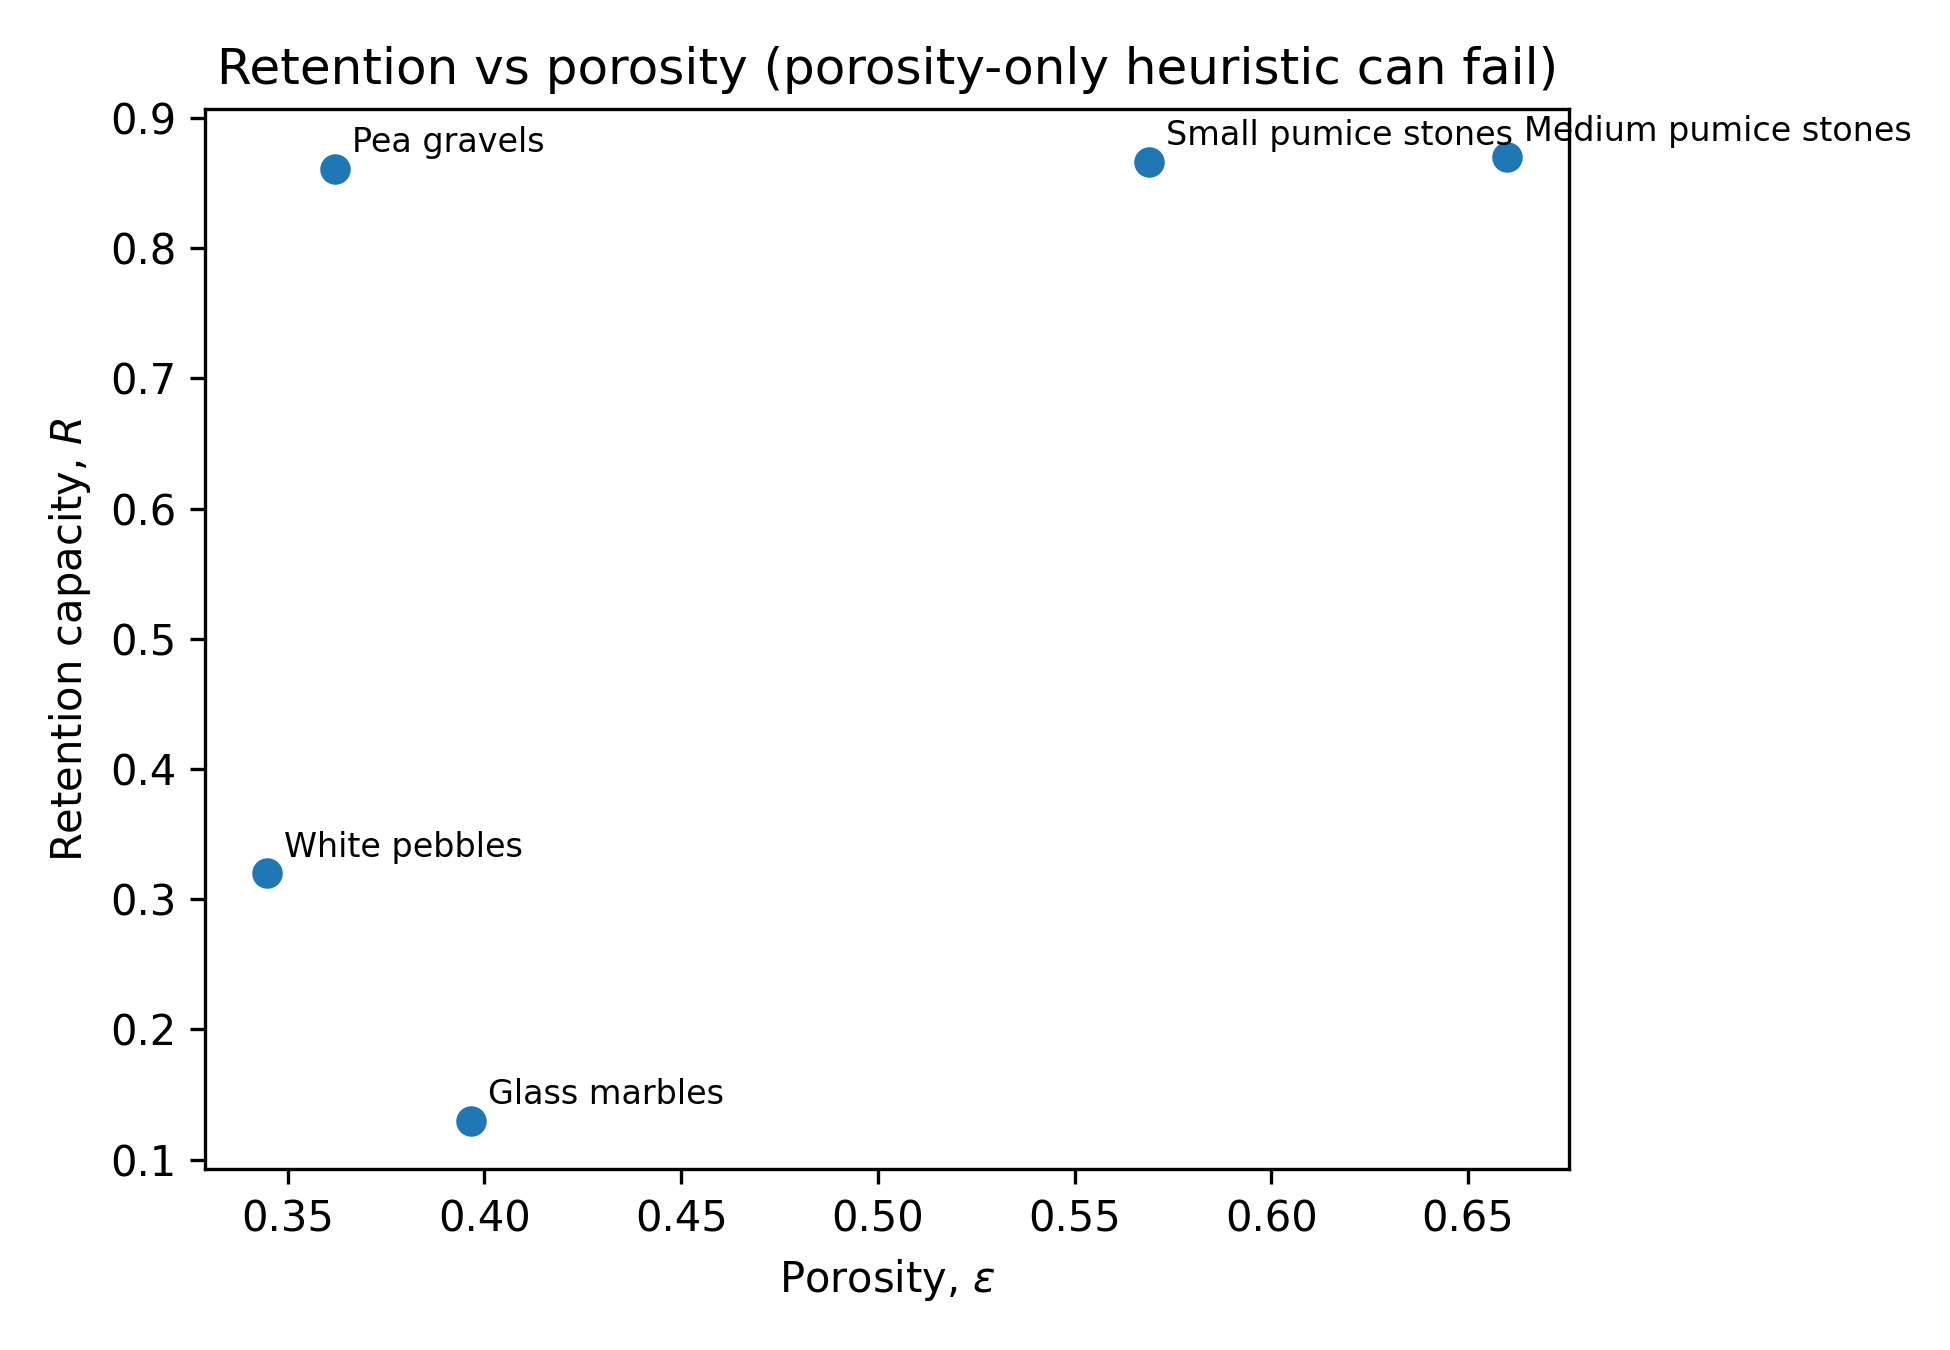
\includegraphics[width=0.8\textwidth]{paper2_outputs/figures/fig_retention_vs_porosity.png}
    \caption{Retention capacity ($R$) versus porosity ($\varepsilon$) across packing media. The relationship is non-monotonic: glass marbles exhibit the lowest retention despite moderate porosity, while pea gravels achieve high retention despite lower porosity. This pattern falsifies a strict volumetric interpretation of biomass retention.}
    \label{fig:retention_vs_porosity}
\end{figure}

\subsection{Stage~I results: hydraulic signatures reveal medium-specific flow resistance}

If porosity does not explain retention, perhaps the hydrodynamic properties of each packing---captured through pressure-drop behaviour---can discriminate between high- and low-retention media. Table~\ref{tab:hydraulic_signature} presents posterior summaries from the Stage~I Bayesian Darcy--Forchheimer calibration, based on $n=240$ pressure-drop measurements (48 velocities per medium) spanning $u=3.9\times 10^{-6}$--$5.0\times 10^{-5}$~m~s$^{-1}$.

The inferred permeability $k$ varied by more than two orders of magnitude across media. Medium pumice stones exhibited the highest permeability ($\hat{k}=1.755\times 10^{-6}$~m$^2$), consistent with their high porosity and open pore structure. Pea gravels exhibited the lowest permeability ($\hat{k}=1.526\times 10^{-8}$~m$^2$), representing a $115\times$ range. Credible intervals for $k$ were tight for several media (e.g., glass marbles: $k \in [1.238, 1.249] \times 10^{-7}$~m$^2$), indicating that the Darcy (linear) contribution was well-identified.

By contrast, the Forchheimer inertial coefficient $\beta$ exhibited wide posterior ranges, consistent with the expectation that the quadratic term is weakly informed in the creeping-to-laminar regime where $u^2$ contributions are small. Critically, pea gravels exhibited a markedly higher posterior mean $\beta$ ($3.37\times10^{5}$) than all other media (typically $\sim2\times10^{3}$--$5\times10^{3}$). This two-orders-of-magnitude difference suggests strong form drag and frictional energy dissipation arising from the irregular packing geometry of pea gravels---precisely the medium that achieved the highest retention despite its low porosity.

Figure~\ref{fig:pressure_drop_fits} demonstrates that posterior predictive curves closely tracked observed pressure-drop relationships across all media, validating the Stage~I calibration. The geometric damping index (GDI), derived from an apparent shape factor $\hat{\Psi}$, collapsed to values near zero for all media ($\widehat{\mathrm{GDI}} \approx 0$), indicating that this particular geometry surrogate did not discriminate between packings in the present mapping. This limitation is addressed in Section~\ref{sec:limitations}.

\begin{table}
\caption{Bayesian hydraulic signature summaries from Darcy--Forchheimer calibration (posterior mean and 95\% credible interval).}
\label{tab:hydraulic_signature}
\resizebox{\textwidth}{!}{%
\begin{tabular}{lrrrrrrrr}
\toprule
Medium & $\hat{k}$ & $k_{2.5\%}$ & $k_{97.5\%}$ & $\hat{\beta}$ & $\beta_{2.5\%}$ & $\beta_{97.5\%}$ & $\hat{\Psi}$ & $\widehat{\mathrm{GDI}}$ \\
\midrule
Glass marbles & 1.241e-07 & 1.238e-07 & 1.249e-07 & 1936 & 1622 & 2878 & 1.004 & 0 \\
Medium pumice stones & 1.755e-06 & 1.24e-06 & 2.826e-06 & 4729 & 1471 & 1.007e+04 & 1.204 & 0 \\
Pea gravels & 1.526e-08 & 1.068e-08 & 2.675e-08 & 3.366e+05 & 7166 & 1.022e+06 & 1.152 & 0 \\
Small pumice stones & 1.419e-07 & 1.402e-07 & 1.463e-07 & 2551 & 953.2 & 6425 & 1.009 & 0 \\
White pebbles & 6.042e-08 & 6.038e-08 & 6.053e-08 & 3022 & 2859 & 3499 & 1.003 & 0 \\
\bottomrule
\end{tabular}
}
\end{table}


\begin{figure}[H]
    \centering
    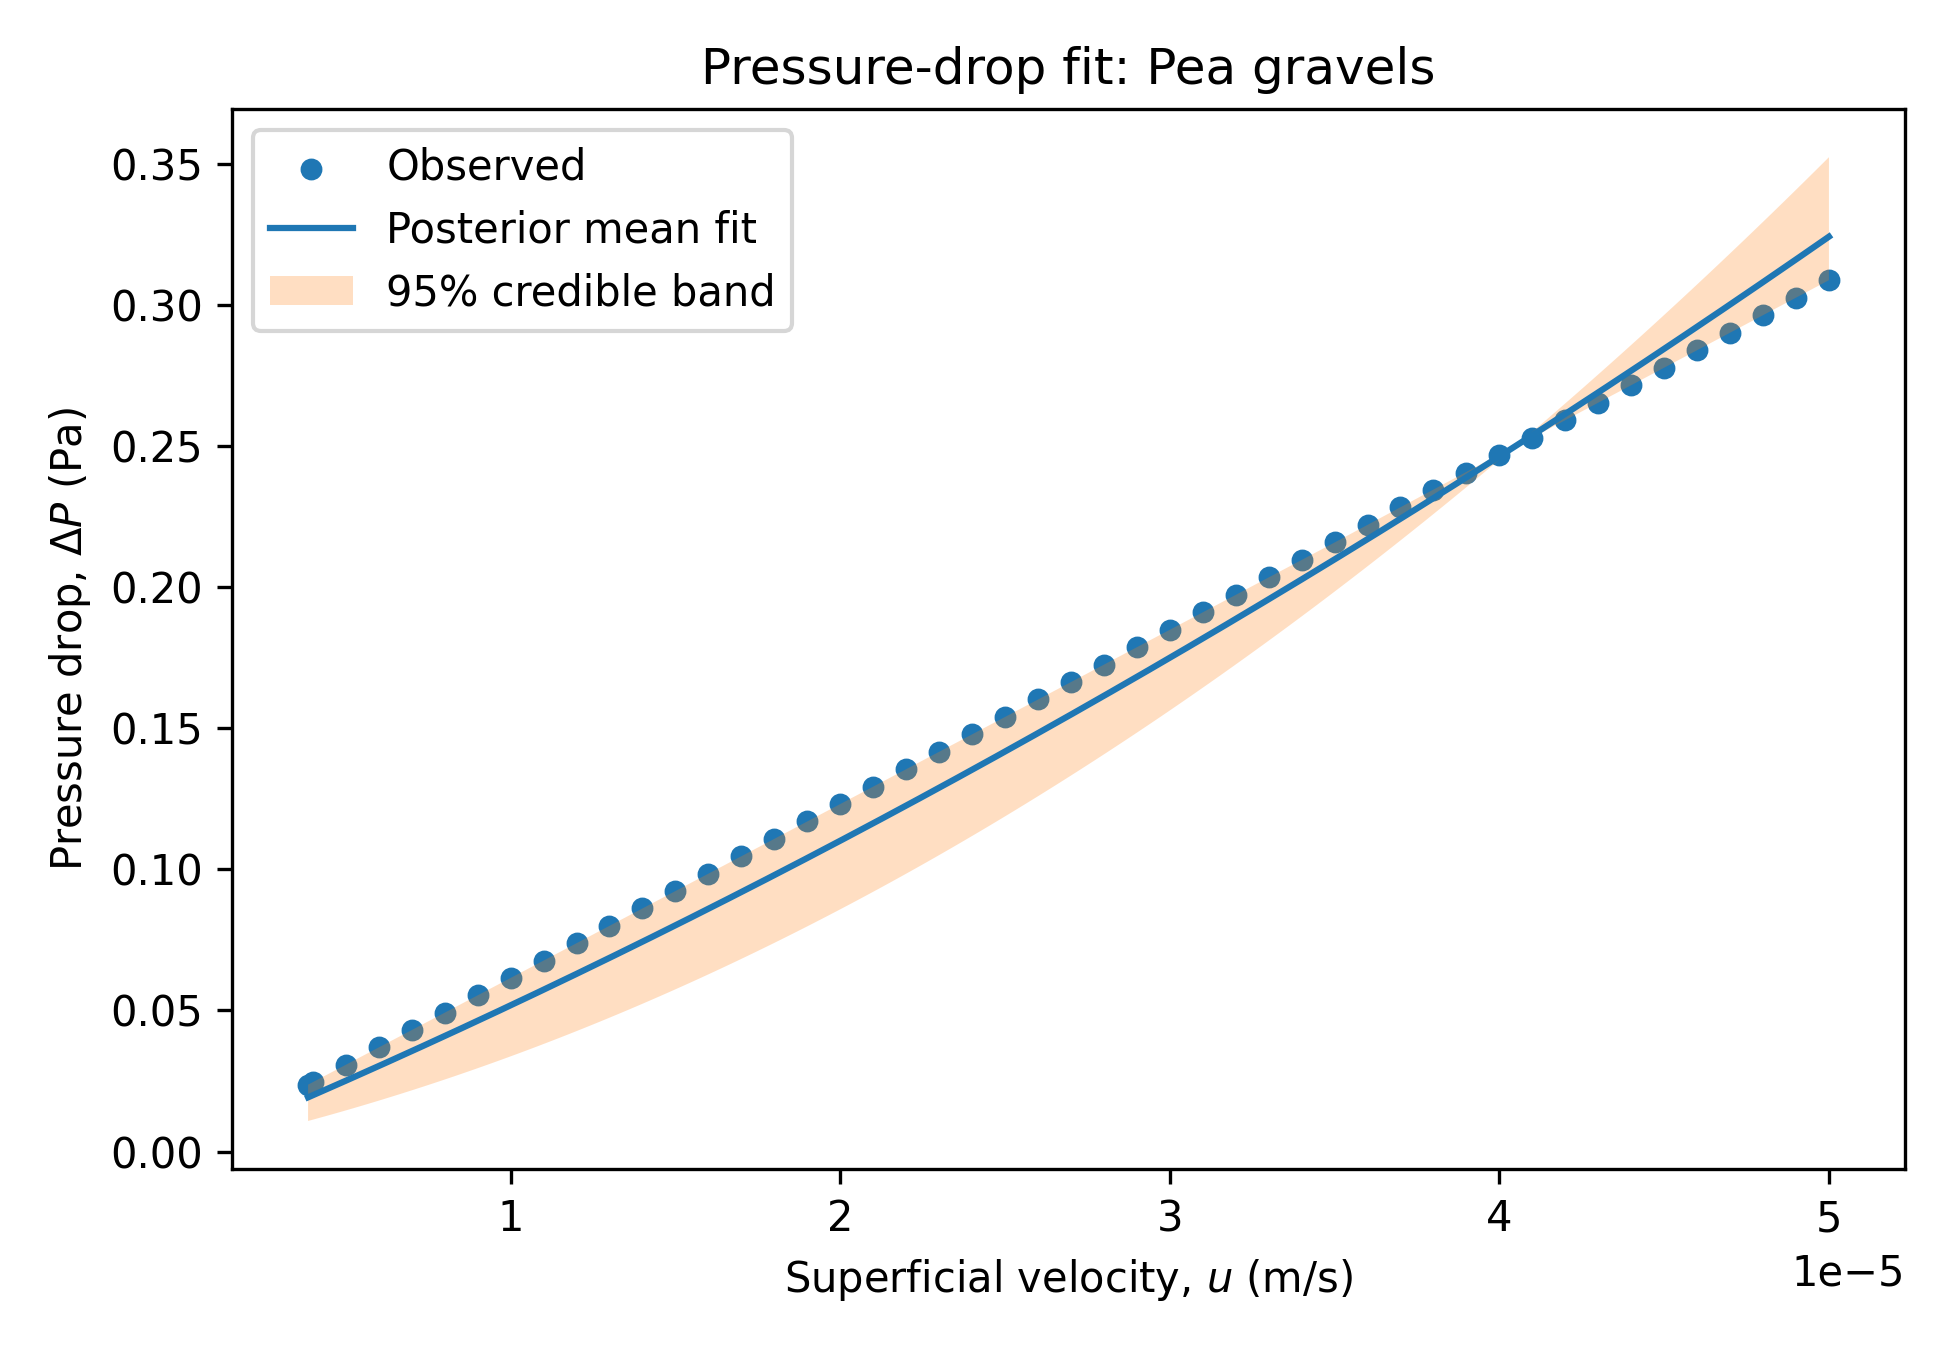
\includegraphics[width=0.48\textwidth]{paper2_outputs/figures/fig_pressure_drop_pea_gravels.png}
    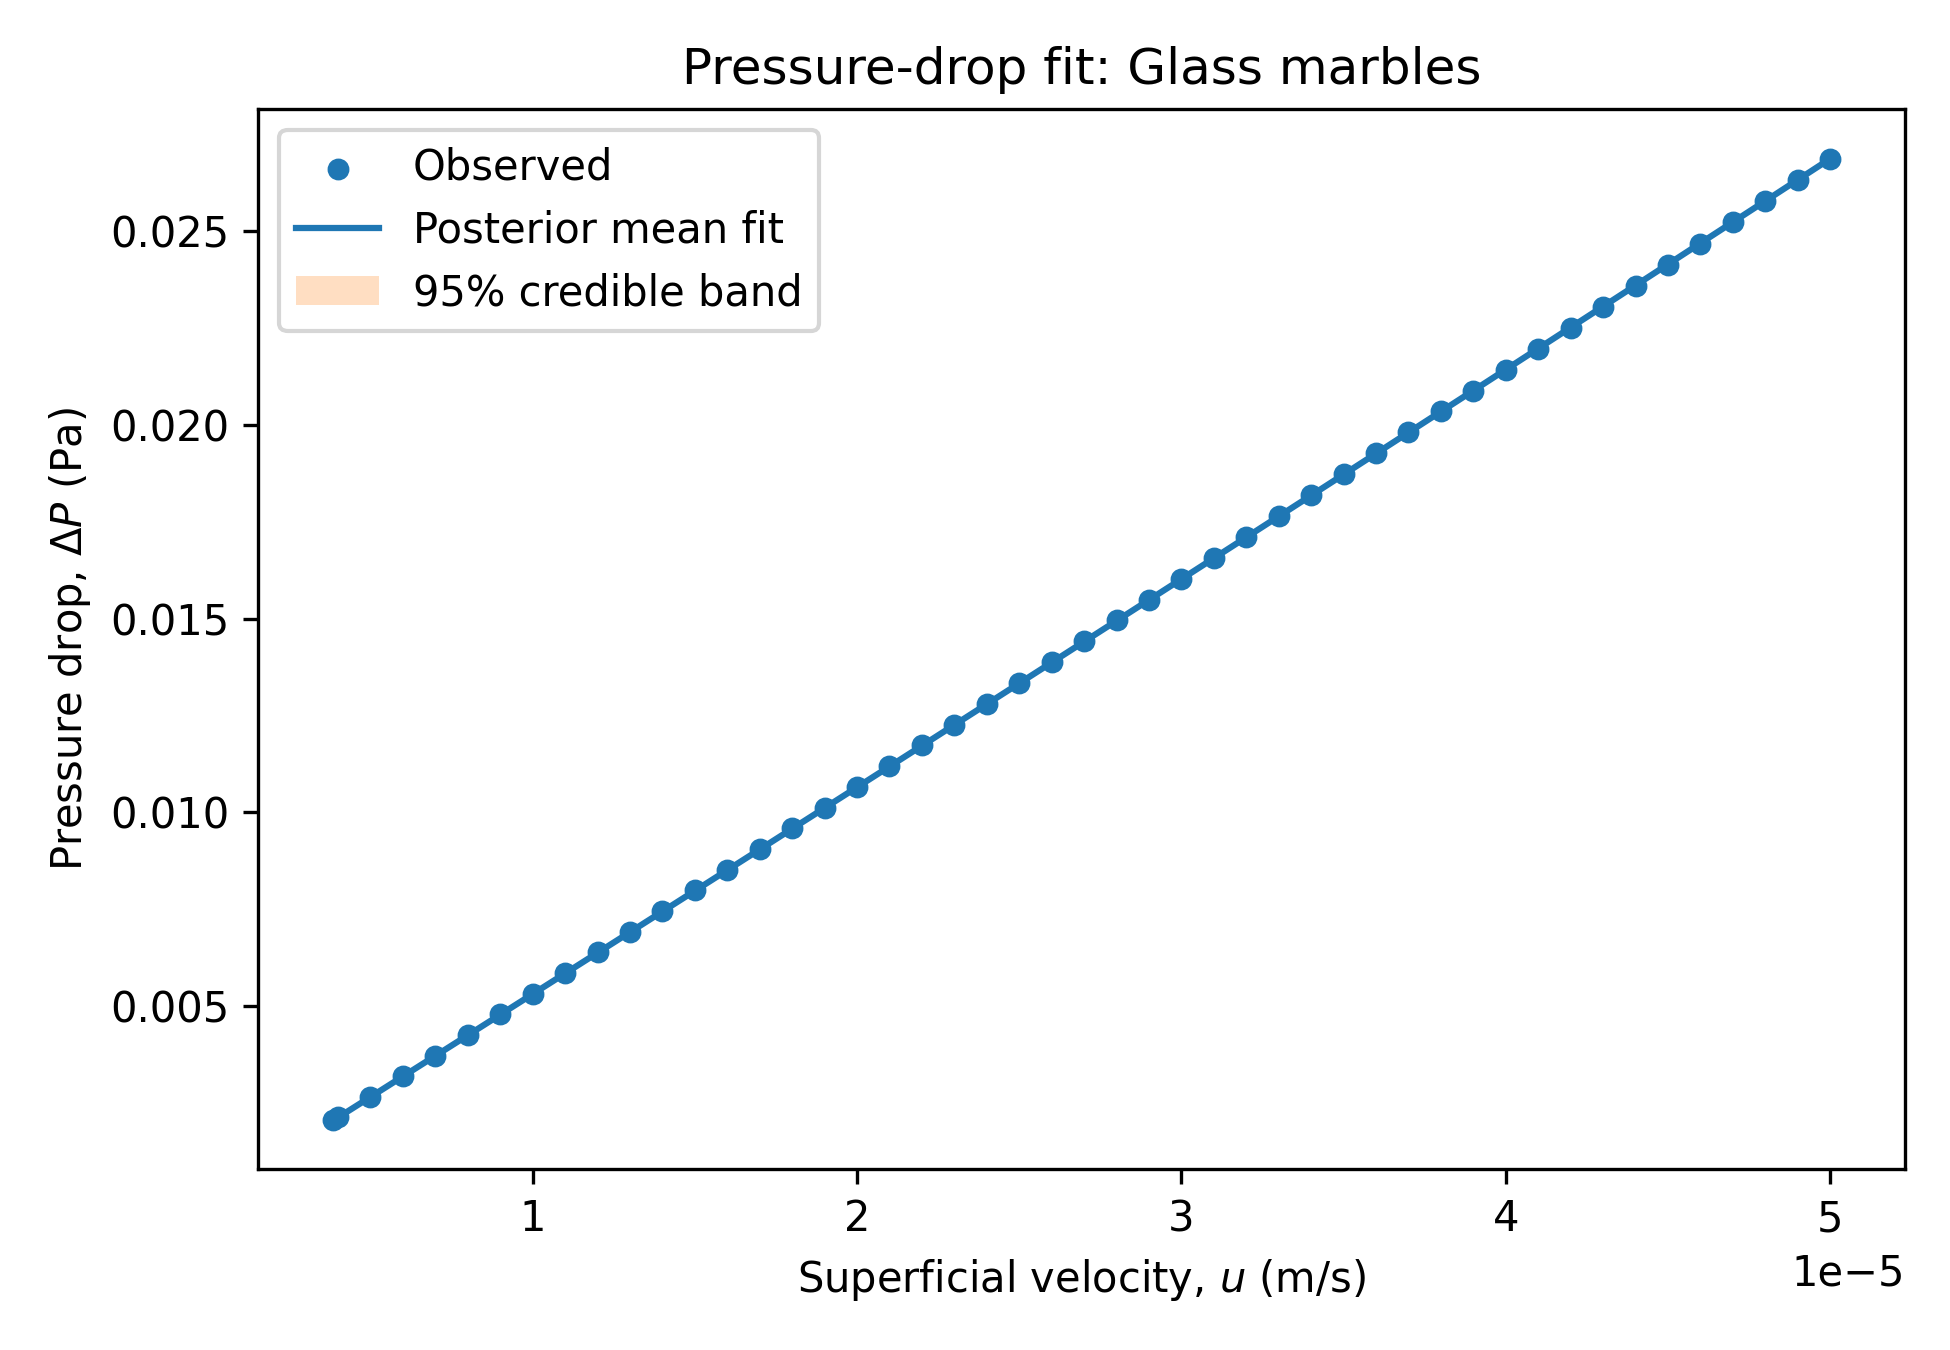
\includegraphics[width=0.48\textwidth]{paper2_outputs/figures/fig_pressure_drop_glass_marbles.png}\\
    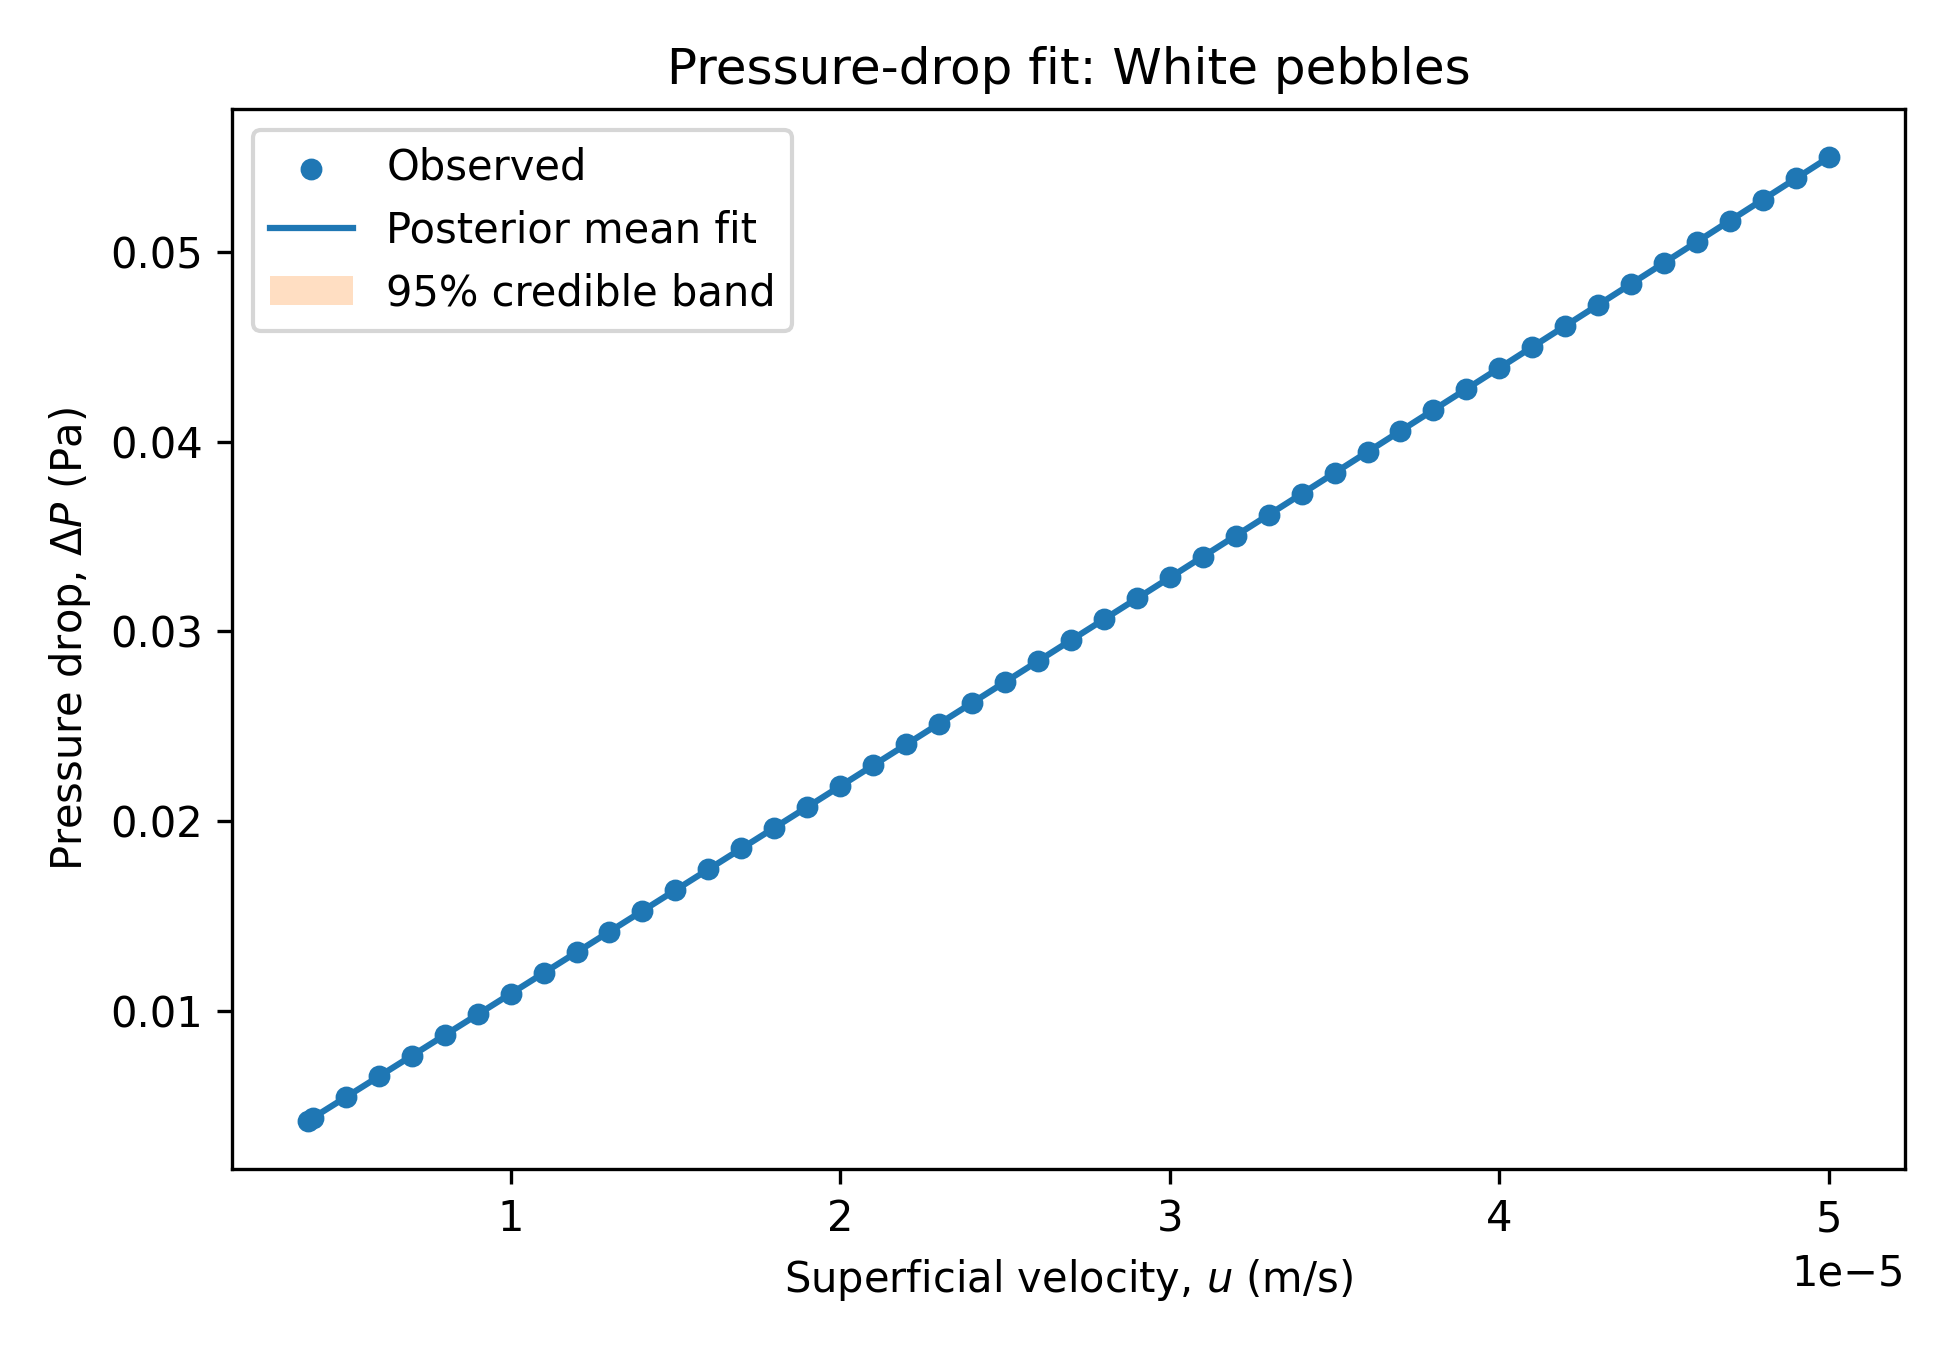
\includegraphics[width=0.48\textwidth]{paper2_outputs/figures/fig_pressure_drop_white_pebbles.png}
    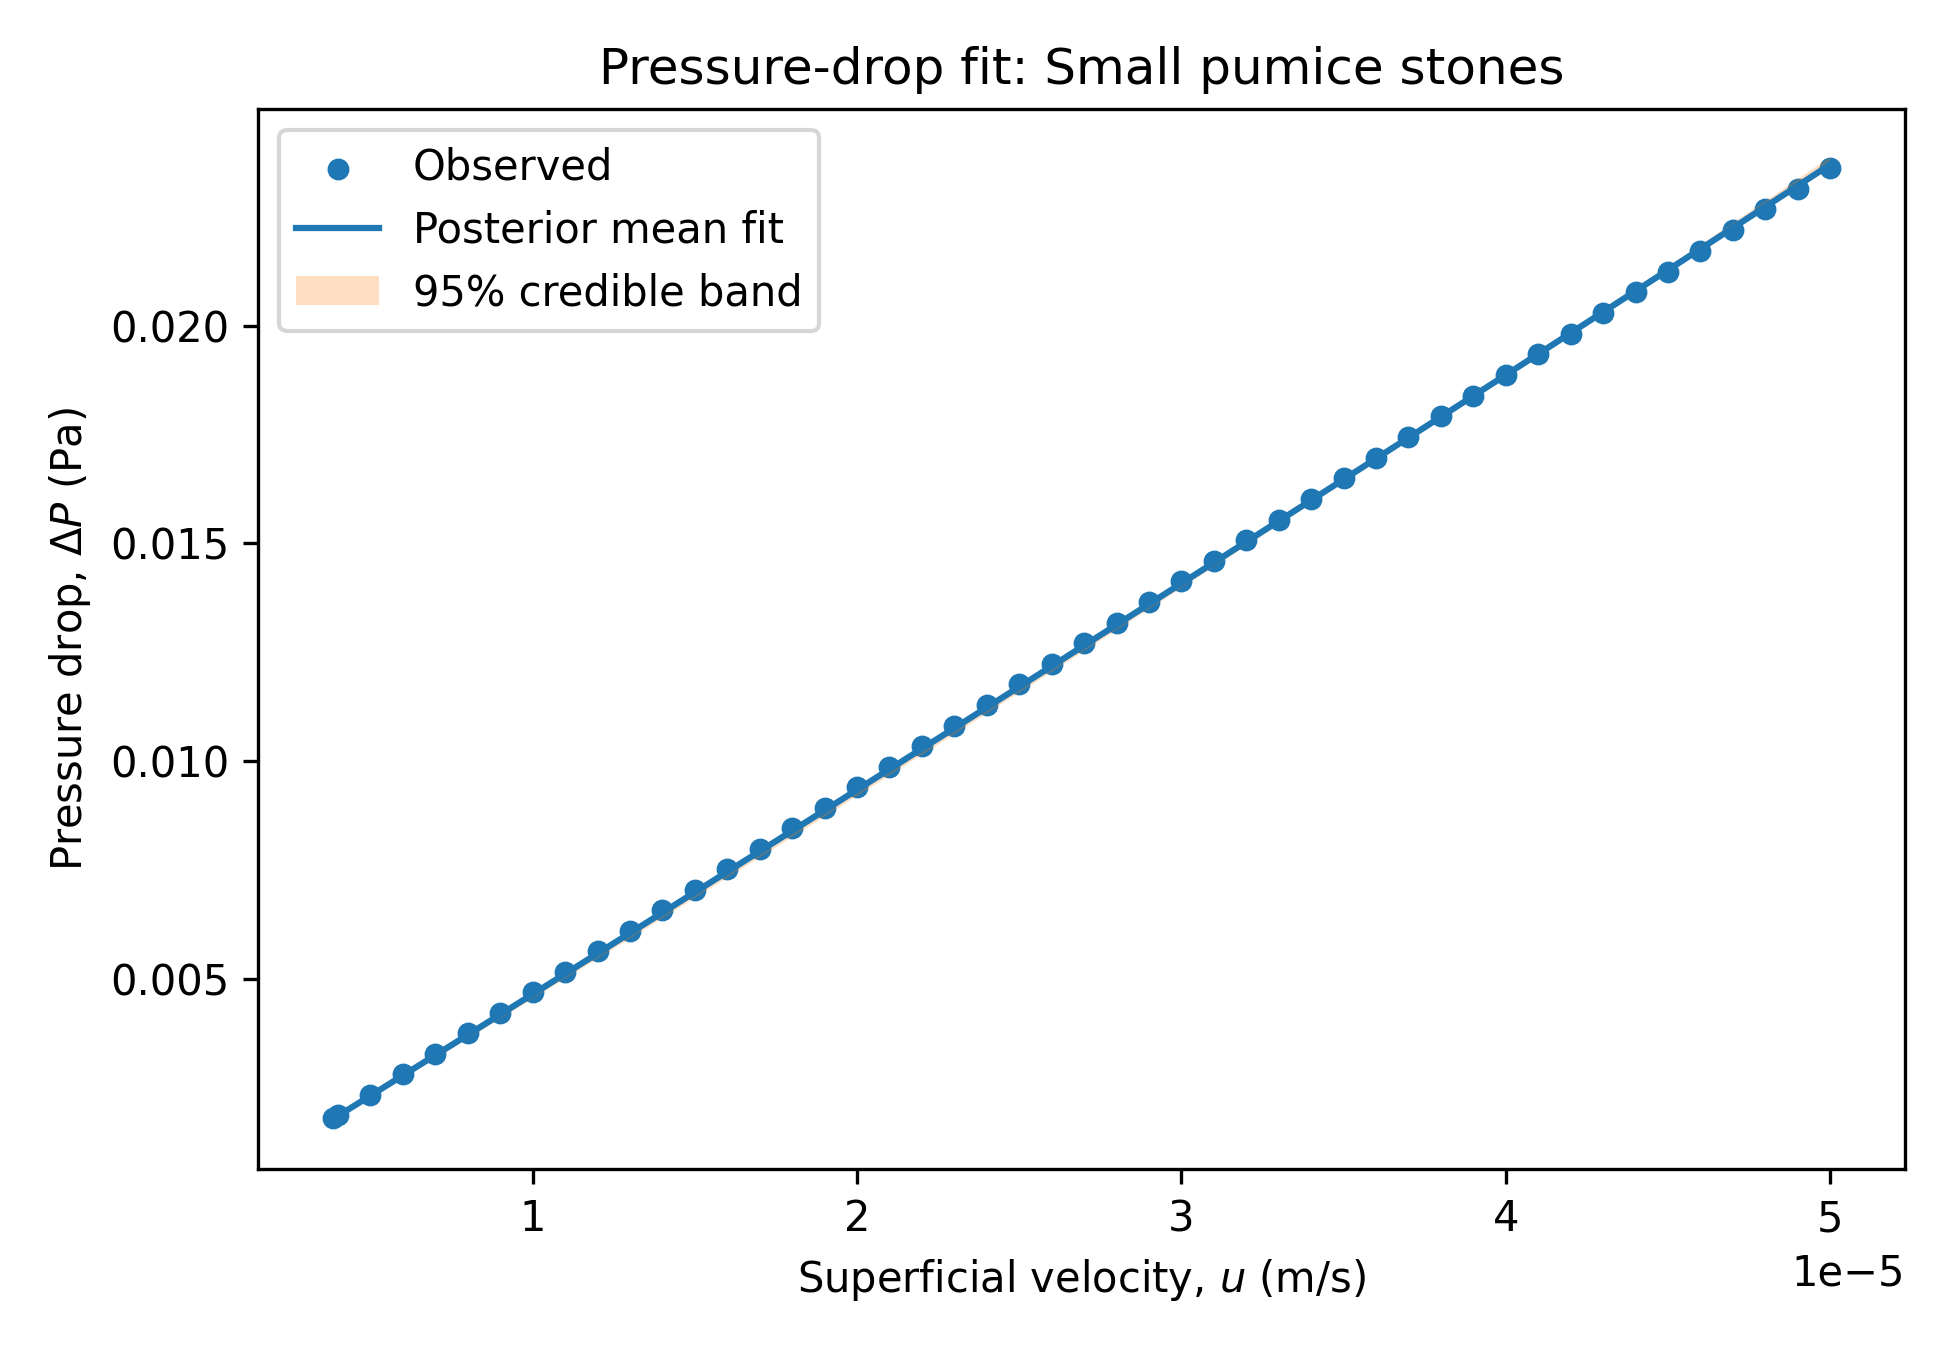
\includegraphics[width=0.48\textwidth]{paper2_outputs/figures/fig_pressure_drop_small_pumice_stones.png}\\
    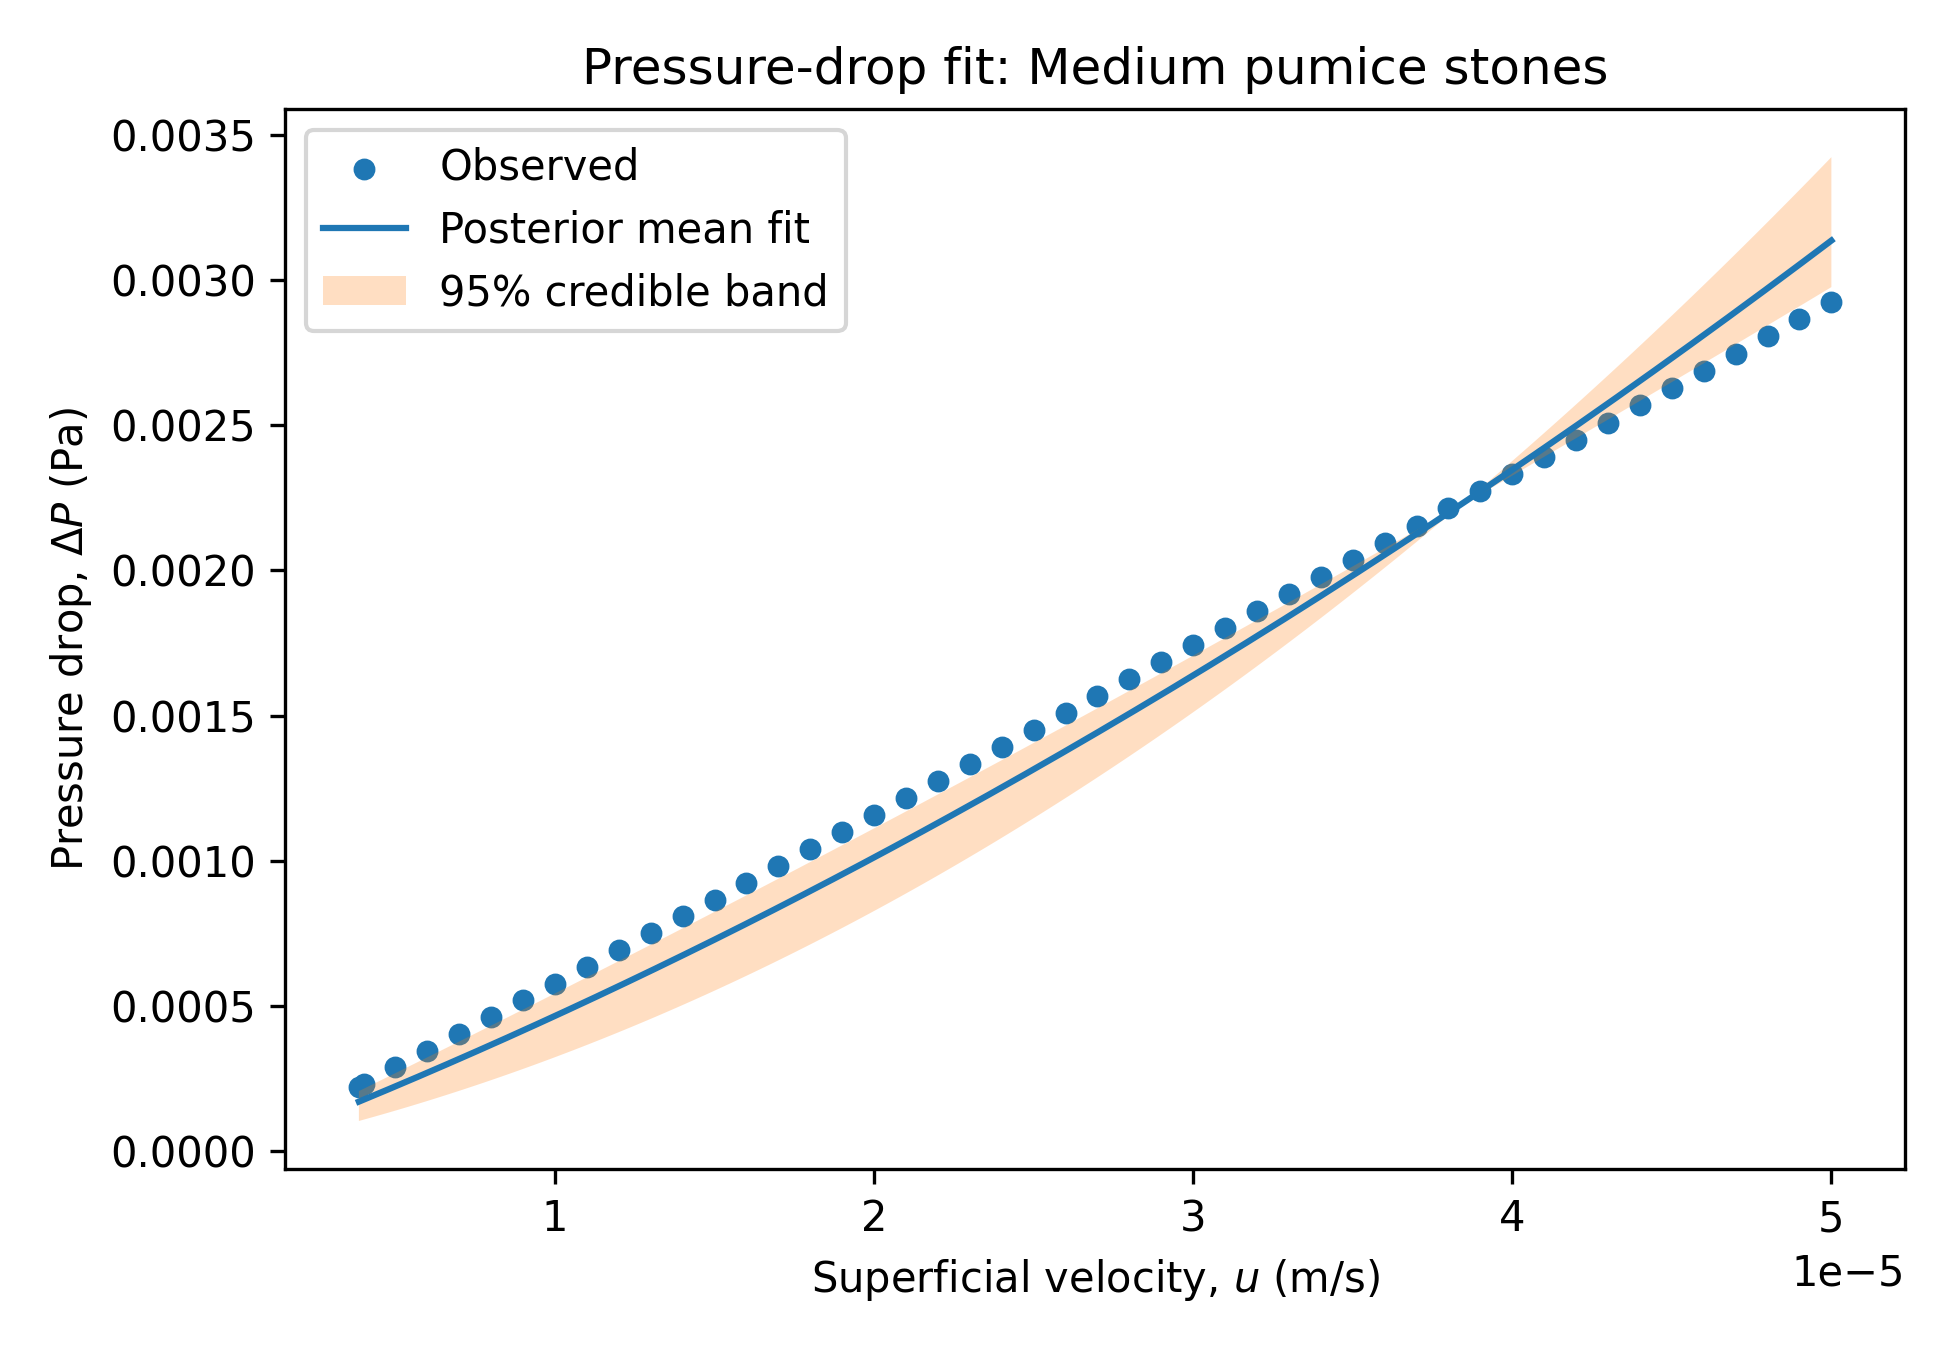
\includegraphics[width=0.48\textwidth]{paper2_outputs/figures/fig_pressure_drop_medium_pumice_stones.png}
    \caption{Posterior predictive fits from Stage~I Bayesian Darcy--Forchheimer calibration. Posterior mean curves (solid lines) and 95\% credible bands (shaded regions) demonstrate close agreement with observed pressure-drop data across all five packing media.}
    \label{fig:pressure_drop_fits}
\end{figure}

\subsection{Stage~II results: competing retention models}

With hydraulic signatures $(k, \beta)$ now available as candidate predictors, we can formally test whether they improve upon the volumetric (porosity-only) hypothesis. Table~\ref{tab:stage2_consolidated} presents regression coefficients for all four competing Beta-regression models side-by-side, enabling direct comparison of effect sizes and posterior sign probabilities.

Several patterns emerge from this comparison. First, the Forchheimer coefficient consistently exhibits the strongest posterior evidence for a positive effect on retention. In the combined model, $P(\beta_{\log(1+\beta_{\mathrm{F}})} > 0) = 0.95$, indicating that higher inertial resistance (form drag) is associated with higher retention with 95\% posterior probability. Second, porosity effects are amplified in the combined model ($\hat{\beta}_{\mathrm{logit}(\varepsilon)} = 0.86$, $P(>0) = 0.88$) relative to the volumetric-only model ($\hat{\beta}_{\mathrm{logit}(\varepsilon)} = 0.65$, $P(>0) = 0.82$), suggesting that porosity contributes unique information about void structure once hydraulic signatures account for flow resistance. Third, the GDI model yields an effectively null slope ($\hat{\beta}_{\log(\mathrm{GDI})} = -0.03$, $P(>0) = 0.43$), confirming that the present geometry surrogate adds no explanatory information beyond an intercept.

The dispersion parameter $\kappa$ increased monotonically from the volumetric model ($\hat{\kappa} = 2.82$) through the hydraulic model ($\hat{\kappa} = 3.37$) to the combined model ($\hat{\kappa} = 4.44$). Since higher $\kappa$ implies tighter concentration of the Beta distribution around its mean, this pattern indicates that incorporating additional predictors progressively reduced unexplained heterogeneity in retention outcomes.

\begin{table}[H]
\caption{Stage~II Bayesian retention model coefficients across competing hypotheses. Posterior means with 95\% highest density intervals (HDI) are shown; $P(>0)$ denotes the posterior probability that the coefficient is positive. The combined model exhibits the strongest evidence for positive effects across all predictors.}
\label{tab:stage2_consolidated}
\centering
\small
\begin{tabular}{lcccc}
\toprule
Parameter & Volumetric & Hydraulic & Combined & GDI \\
\midrule
Intercept ($\alpha$) & 0.43 & 0.42 & $-0.12$ & 0.01 \\
 & [$-0.56$, $1.36$] & [$-3.20$, $4.16$] & [$-3.53$, $3.67$] & [$-3.98$, $3.82$] \\[0.5em]
$\beta_{\mathrm{logit}(\varepsilon)}$ & 0.65 & --- & 0.86 & --- \\
 & [$-0.88$, $1.98$] & & [$-0.52$, $2.32$] & \\
 & $P(>0)=0.82$ & & $P(>0)=0.88$ & \\[0.5em]
$\beta_{\log k}$ & --- & 0.26 & 0.23 & --- \\
 & & [$-0.17$, $0.68$] & [$-0.16$, $0.64$] & \\
 & & $P(>0)=0.88$ & $P(>0)=0.88$ & \\[0.5em]
$\beta_{\log(1+\beta_{\mathrm{F}})}$ & --- & 0.47 & 0.49 & --- \\
 & & [$-0.19$, $1.11$] & [$-0.16$, $1.09$] & \\
 & & $P(>0)=0.92$ & $P(>0)=0.95$ & \\[0.5em]
$\beta_{\log(\mathrm{GDI})}$ & --- & --- & --- & $-0.03$ \\
 & & & & [$-0.34$, $0.24$] \\
 & & & & $P(>0)=0.43$ \\[0.5em]
$\kappa$ (dispersion) & 2.82 & 3.37 & 4.44 & 2.43 \\
 & [$0.63$, $5.79$] & [$0.57$, $6.67$] & [$0.80$, $8.98$] & [$0.40$, $4.75$] \\
\bottomrule
\end{tabular}
\end{table}


Figure~\ref{fig:forest_all_models} visualizes these coefficient estimates with their 95\% highest density intervals. The combined model exhibits the tightest clustering of positive coefficients, while the GDI model shows a coefficient centered precisely at zero.

\begin{figure}[H]
    \centering
    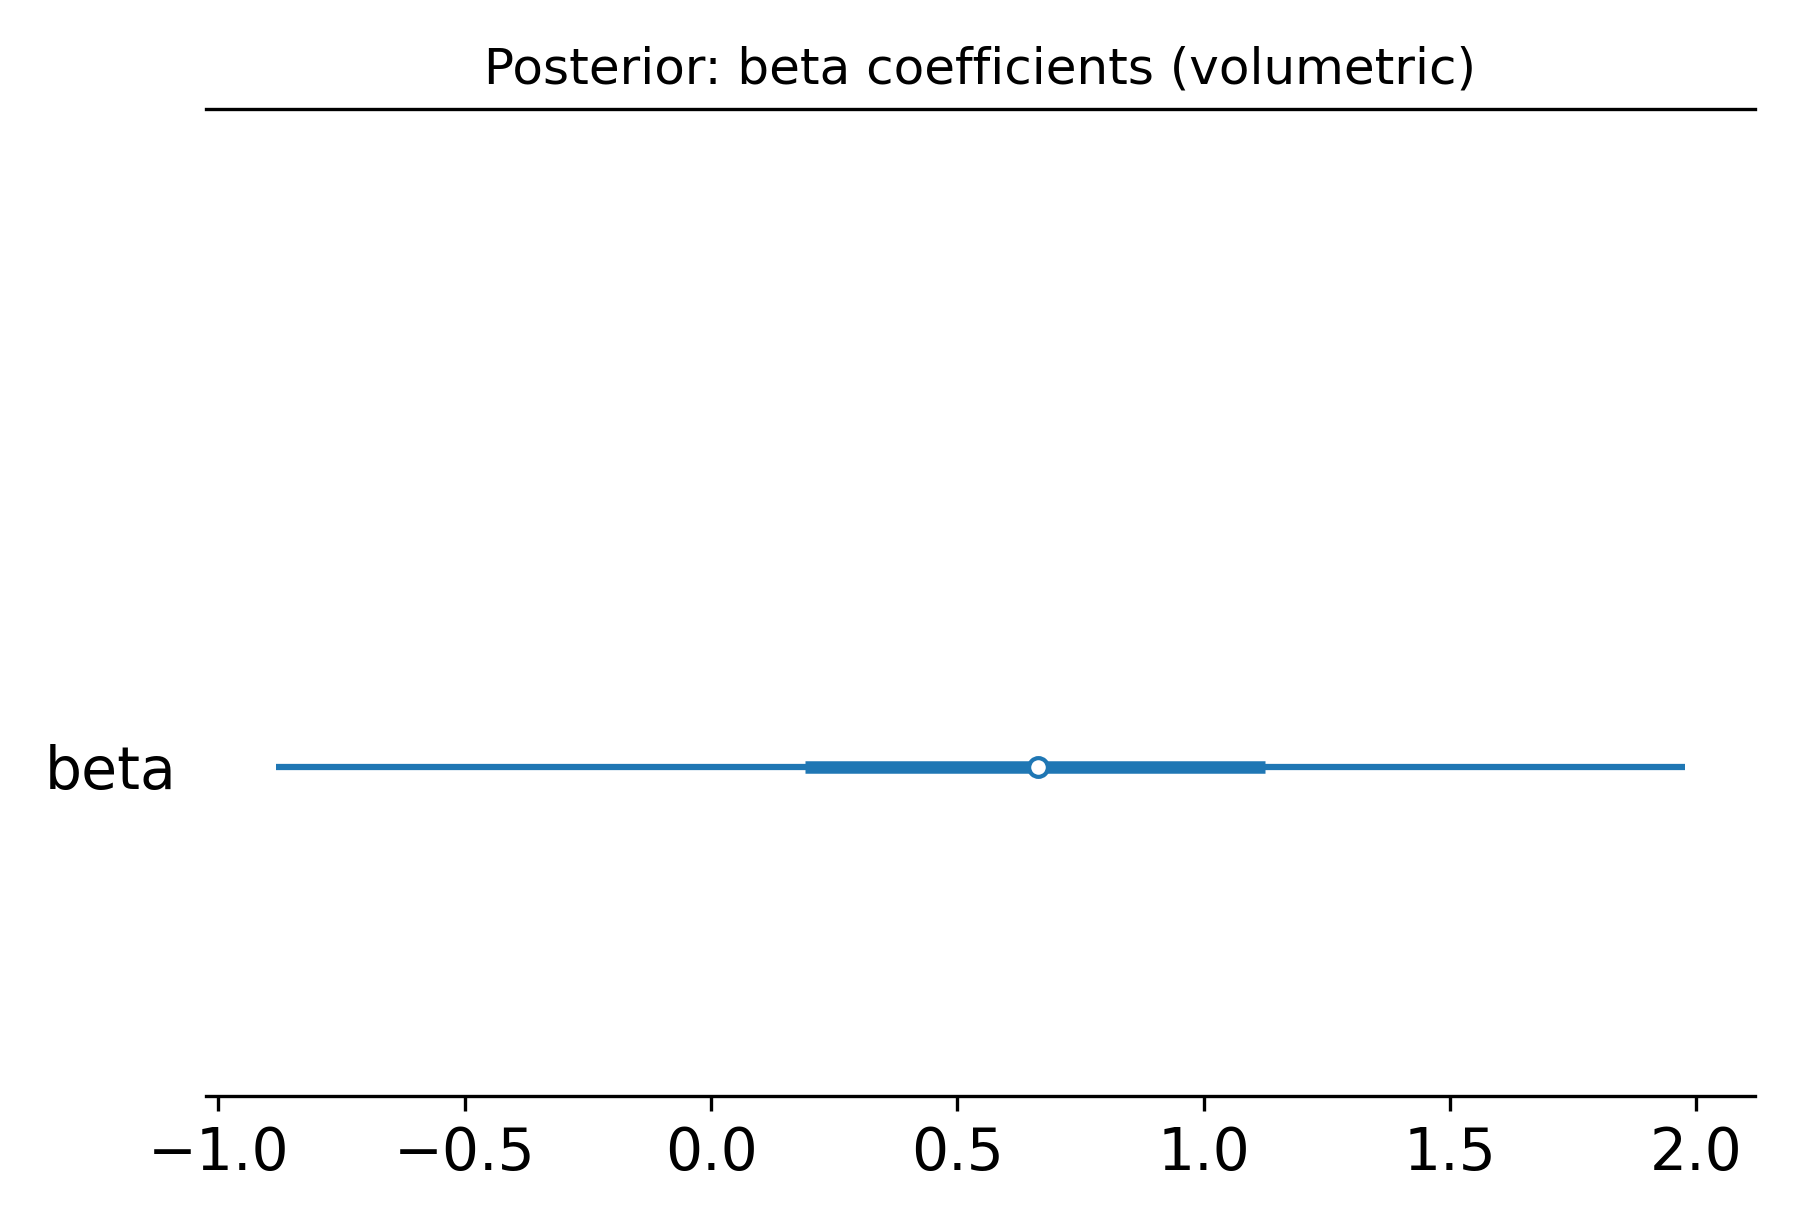
\includegraphics[width=0.48\textwidth]{paper2_outputs/figures/fig_forest_beta_volumetric.png}
    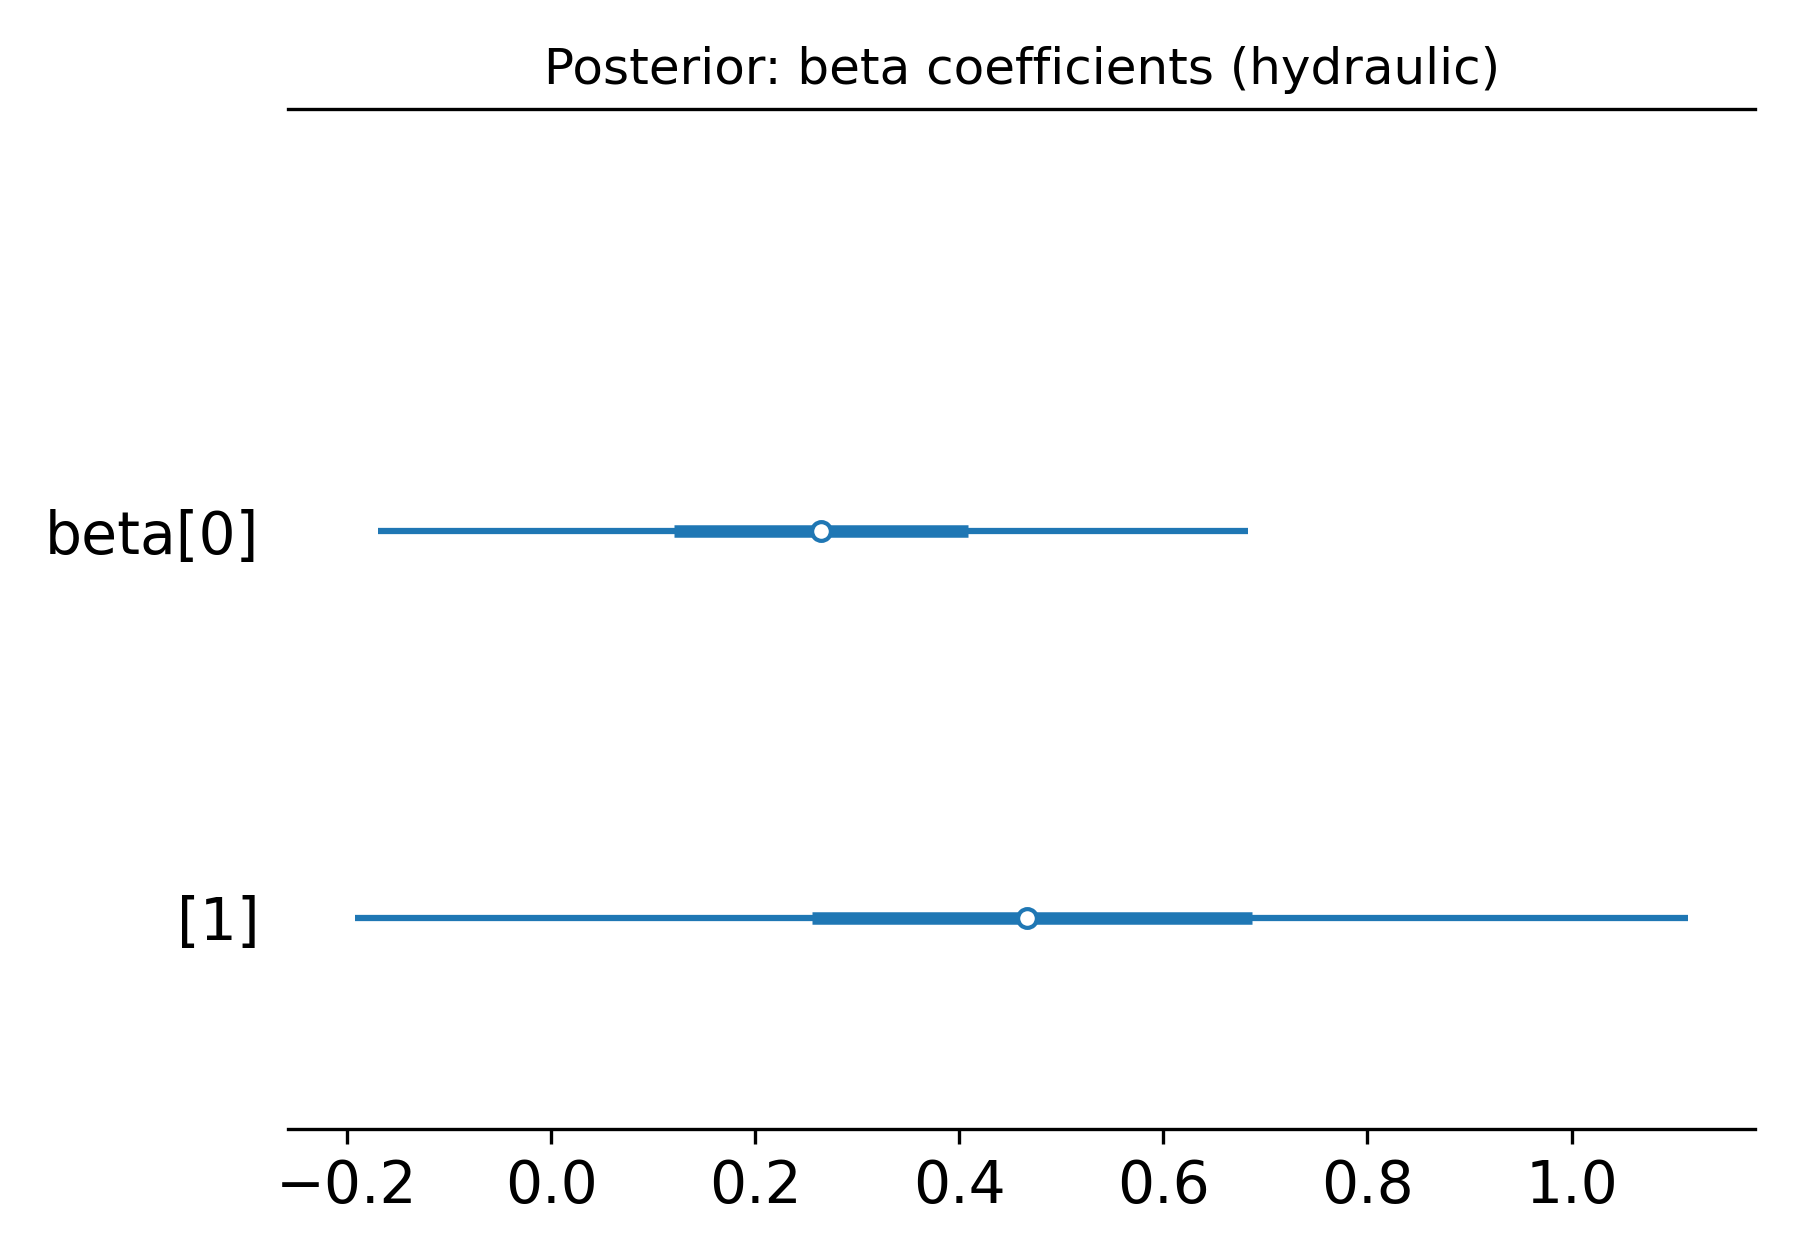
\includegraphics[width=0.48\textwidth]{paper2_outputs/figures/fig_forest_beta_hydraulic.png}\\
    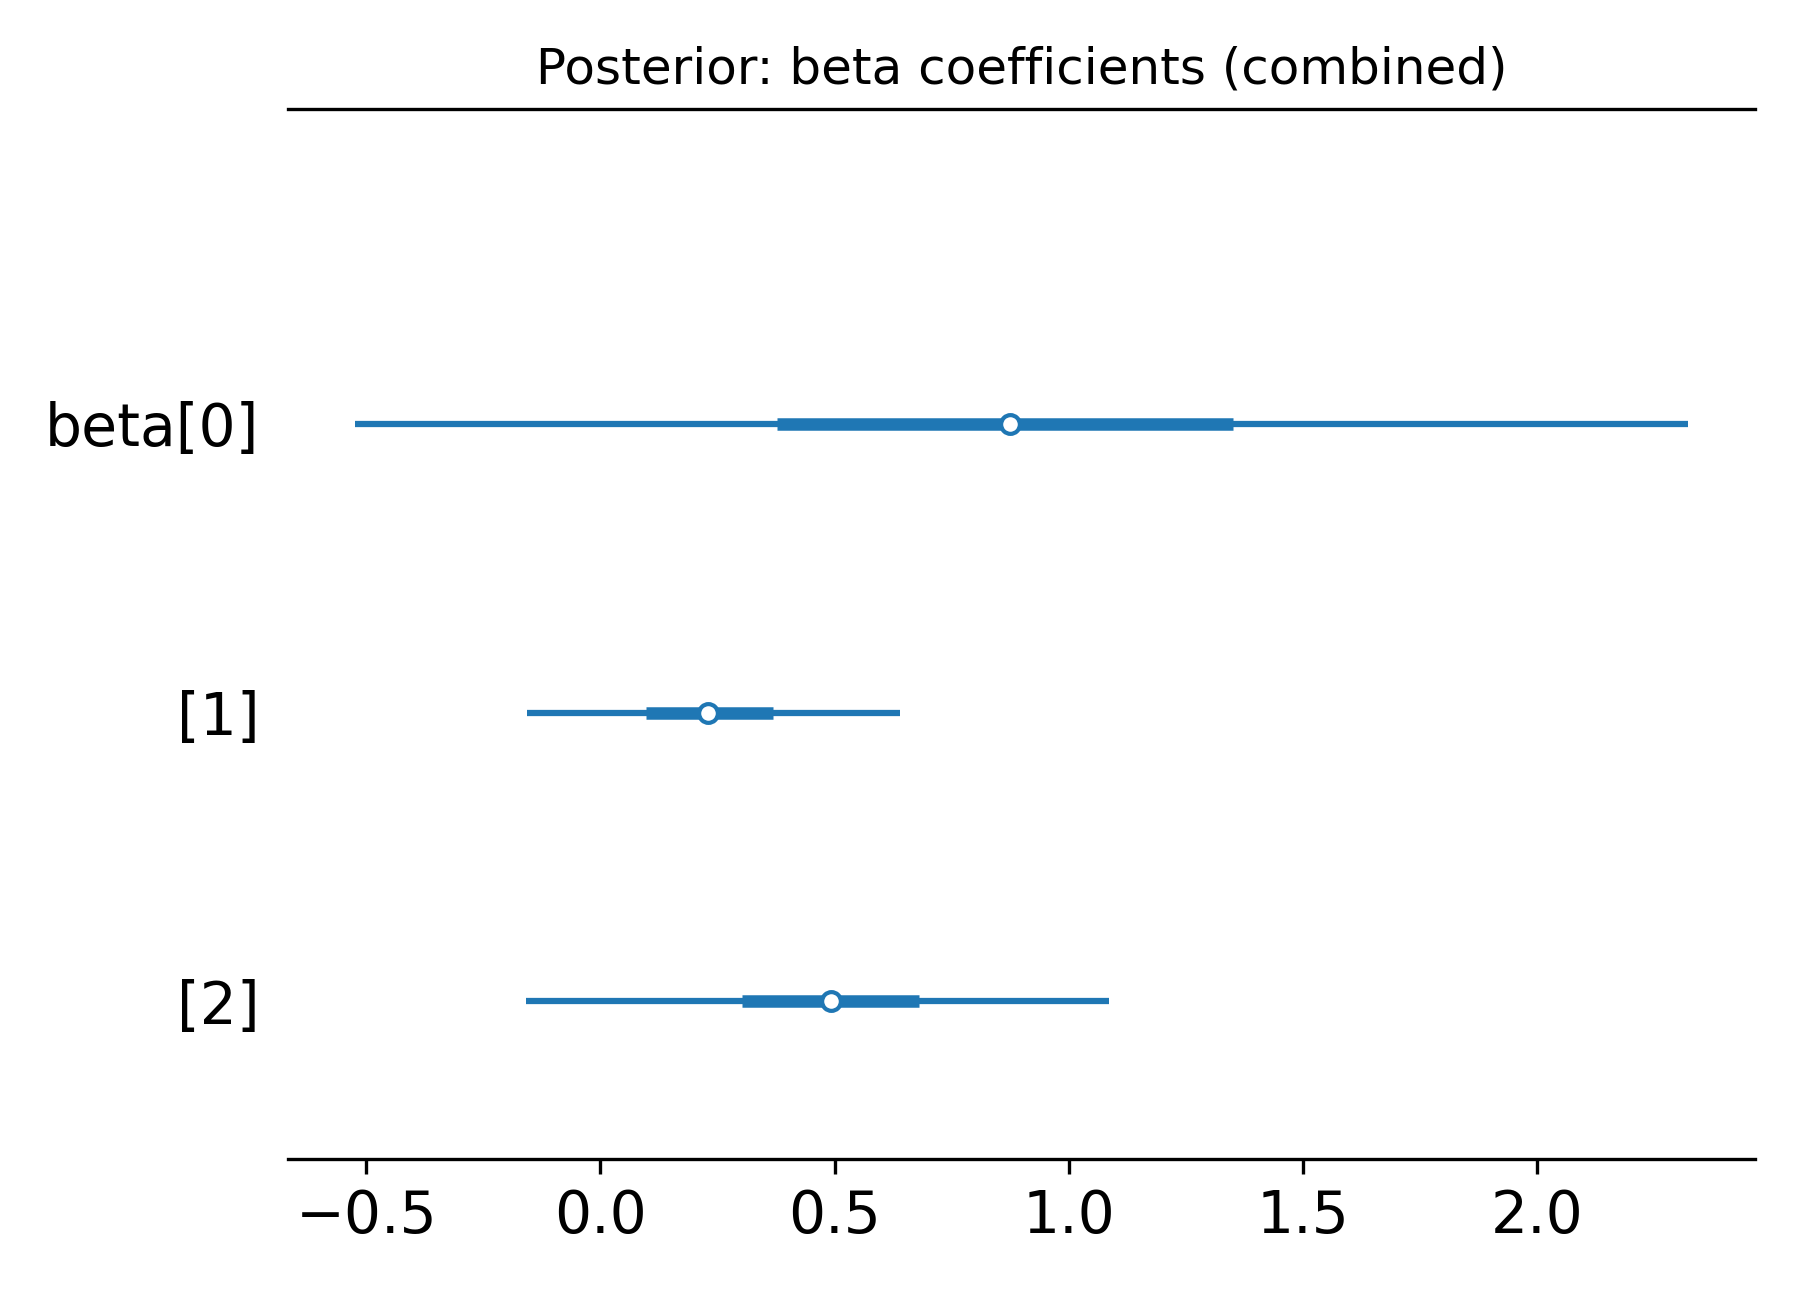
\includegraphics[width=0.48\textwidth]{paper2_outputs/figures/fig_forest_beta_combined.png}
    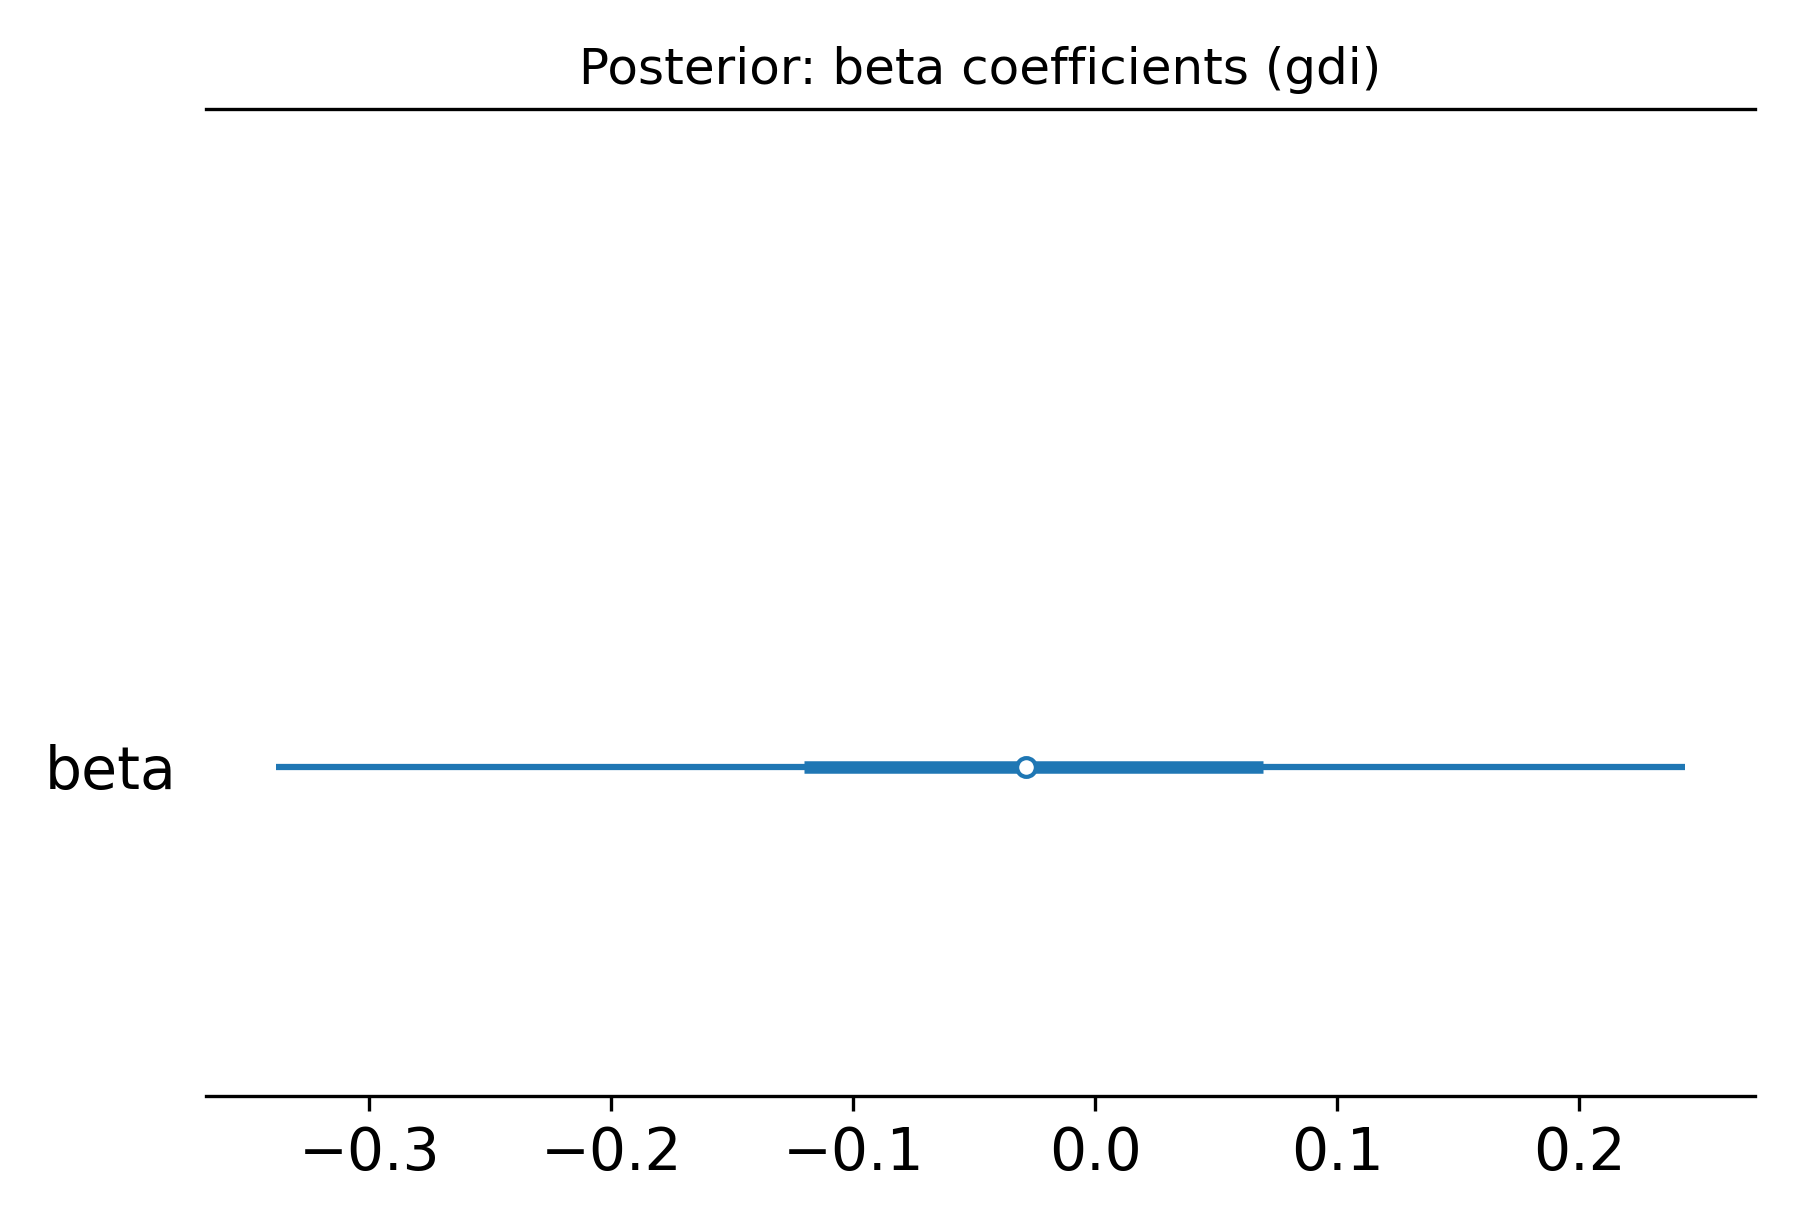
\includegraphics[width=0.48\textwidth]{paper2_outputs/figures/fig_forest_beta_gdi.png}
    \caption{Posterior distributions for regression coefficients across competing Stage~II models. Top left: volumetric (porosity-only). Top right: hydraulic ($\log k$ and $\log(1+\beta_{\mathrm{F}})$). Bottom left: combined. Bottom right: GDI-only. The combined model shows the strongest evidence for positive effects; the GDI model shows a null coefficient.}
    \label{fig:forest_all_models}
\end{figure}

\subsection{Model comparison: predictive evidence from cross-validation}

Coefficient estimates reveal associations, but the decisive test of competing hypotheses is out-of-sample predictive performance. Table~\ref{tab:model_comparison} presents PSIS-LOO cross-validation results. The combined model achieved the highest expected log predictive density ($\mathrm{ELPD}_{\mathrm{LOO}} = -0.995$, SE $= 0.94$) and the largest pseudo-BMA weight (0.40), followed by the volumetric model (ELPD $= -1.691$, weight $= 0.23$), GDI (ELPD $= -1.862$, weight $= 0.19$), and hydraulic-only (ELPD $= -1.872$, weight $= 0.18$).

The ELPD differences relative to the combined model are modest ($\Delta_{\mathrm{ELPD}} \approx 0.7$--$0.9$) with large standard errors, which is expected given only five packing media. Pareto-$k$ diagnostic warnings for the combined and GDI models indicate influential observations. The appropriate interpretation is therefore not decisive model selection, but rather \emph{probabilistic evidence} that combining porosity with hydraulic signatures improves predictive adequacy compared with porosity alone.

\begin{table}
\caption{PSIS-LOO comparison of retention models (higher ELPD indicates better expected predictive performance).}
\label{tab:model_comparison}
\begin{tabular}{lrrrr}
\toprule
Model & ELPD$_{\mathrm{LOO}}$ & $p_{\mathrm{LOO}}$ & Weight & SE \\
\midrule
combined & -0.9949 & 2.862 & 0.3981 & 0.9385 \\
volumetric & -1.691 & 2.133 & 0.2339 & 1.09 \\
gdi & -1.862 & 1.699 & 0.1886 & 1.19 \\
hydraulic & -1.872 & 2.708 & 0.1795 & 1.154 \\
\bottomrule
\end{tabular}
\end{table}


Table~\ref{tab:retention_predictions} reveals where models succeed and fail. The volumetric model predicted broadly similar mean retention across all media ($\hat{\mu} = 0.50$--$0.69$), substantially over-predicting the low-retention smooth media: for glass marbles, observed $R = 0.130$ versus predicted $\hat{\mu} = 0.537$ (95\% CI: $0.290$--$0.772$). The combined model correctly separated smooth from frictional media: glass marbles ($\hat{\mu} = 0.403$), white pebbles ($\hat{\mu} = 0.373$), pea gravels ($\hat{\mu} = 0.776$), and medium pumice ($\hat{\mu} = 0.799$). The GDI model produced identical predictions for all media ($\hat{\mu} = 0.589$), confirming its complete inability to discriminate.

\begin{table}
\caption{Observed retention capacity $R$ and posterior mean retention $\hat\mu$ (95\% credible interval) under the competing Stage II models.}
\label{tab:retention_predictions}
\resizebox{\textwidth}{!}{%
\begin{tabular}{lrrrrr}
\toprule
Medium & Observed $R$ & $\hat\mu$ (volumetric) & $\hat\mu$ (hydraulic) & $\hat\mu$ (combined) & $\hat\mu$ (gdi) \\
\midrule
Pea gravels & 0.861 & 0.514 (0.252--0.778) & 0.796 (0.415--0.984) & 0.776 (0.378--0.980) & 0.589 (0.330--0.810) \\
White pebbles & 0.320 & 0.503 (0.234--0.780) & 0.459 (0.195--0.759) & 0.373 (0.149--0.688) & 0.589 (0.330--0.810) \\
Glass marbles & 0.130 & 0.537 (0.290--0.772) & 0.455 (0.193--0.749) & 0.403 (0.181--0.685) & 0.589 (0.330--0.810) \\
Small pumice stones & 0.867 & 0.639 (0.370--0.838) & 0.493 (0.237--0.750) & 0.580 (0.288--0.815) & 0.589 (0.330--0.810) \\
Medium pumice stones & 0.870 & 0.685 (0.334--0.901) & 0.698 (0.407--0.900) & 0.799 (0.476--0.963) & 0.589 (0.330--0.810) \\
\bottomrule
\end{tabular}
}
\end{table}


Figure~\ref{fig:retention_vs_k} illustrates the non-monotonic relationship between permeability and retention. Both low-permeability media (pea gravels) and high-permeability media (medium pumice) achieve high retention, while moderate-permeability glass marbles exhibit the lowest retention. This pattern underscores that hydraulic conductivity alone does not govern retention; surface geometry and form drag are critical.

\begin{figure}[H]
    \centering
    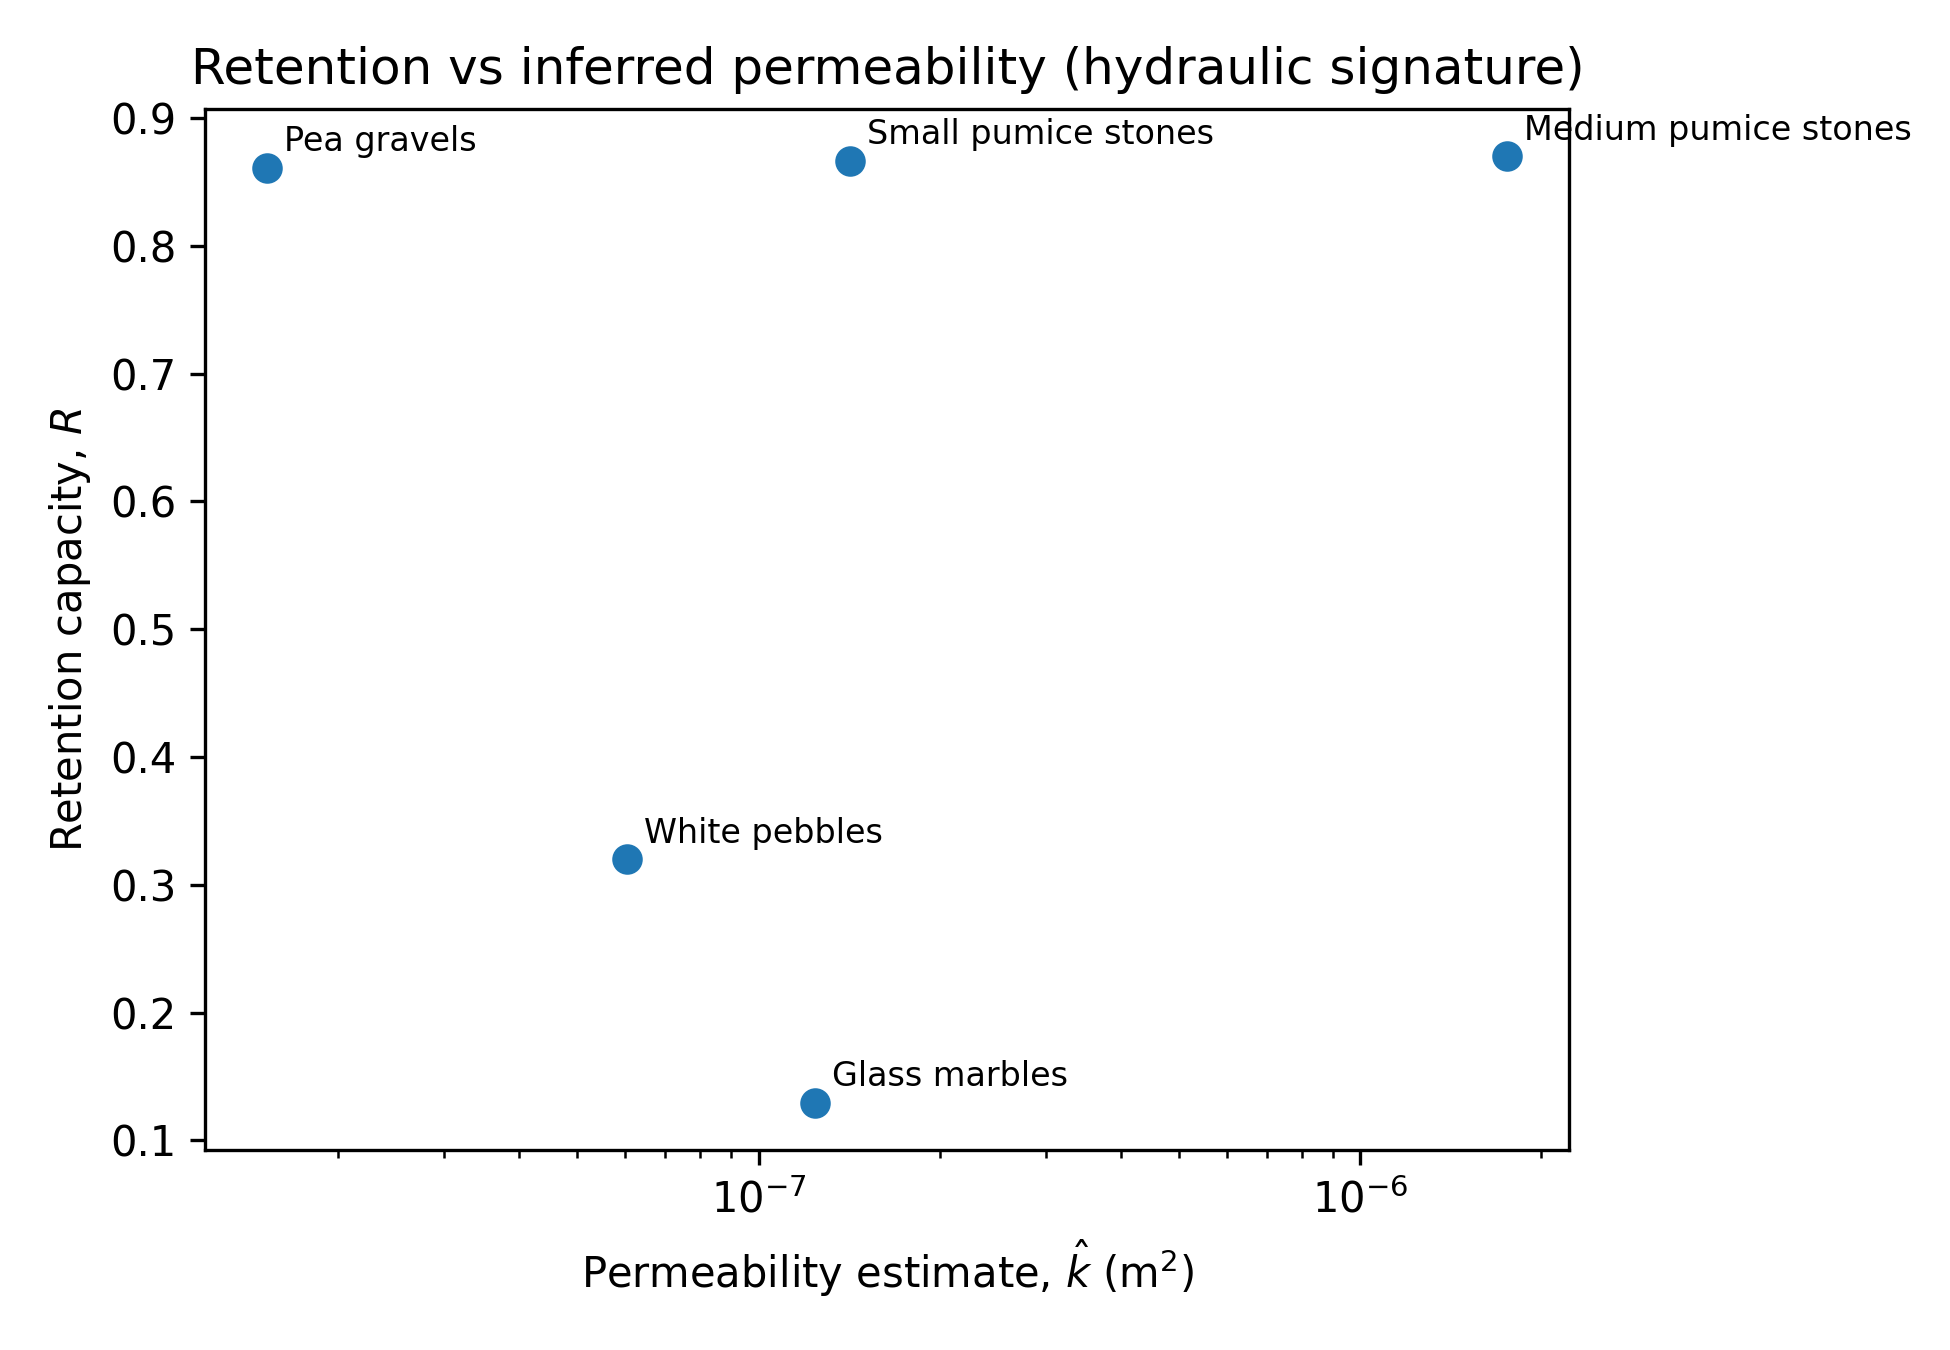
\includegraphics[width=0.7\textwidth]{paper2_outputs/figures/fig_retention_vs_k.png}
    \caption{Retention capacity versus Stage~I posterior mean permeability. The non-monotonic pattern---high retention at both low $k$ (pea gravels) and high $k$ (medium pumice), but low retention at moderate $k$ (glass marbles)---reinforces the friction-limited interpretation.}
    \label{fig:retention_vs_k}
\end{figure}

\subsection{Posterior ranking probabilities for design decisions}

The methodology promised decision-relevant posterior rankings rather than deterministic indices. Table~\ref{tab:posterior_rankings} delivers on this promise by presenting the probability that each medium ranks among the top performers under the combined model. Medium pumice stones and pea gravels dominate the top rankings, with $\Pr(\mathrm{Rank}=1) = 0.42$ and $0.38$ respectively, and $\Pr(\mathrm{Top\text{-}2}) > 0.68$ for both. Glass marbles, by contrast, has only $\Pr(\mathrm{Rank}=1) = 0.02$ and $\Pr(\mathrm{Bottom\text{-}2}) = 0.68$.

These probabilities propagate uncertainty from both Stage~I hydraulic calibration and Stage~II retention modelling, providing a principled basis for material selection under uncertainty. No medium achieves $\Pr(\mathrm{Rank}=1) = 1$, appropriately reflecting the finite sample size and overlapping credible intervals.

\begin{table}[H]
\caption{Posterior ranking probabilities under the combined model. $\Pr(\mathrm{Rank}=1)$ denotes the probability that a medium has the highest predicted retention; $\Pr(\mathrm{Top\text{-}2})$ and $\Pr(\mathrm{Top\text{-}3})$ denote probabilities of being among the top two or three performers; $\Pr(\mathrm{Bottom\text{-}2})$ denotes probability of being among the two lowest performers. Rankings are computed from posterior predictive draws and propagate uncertainty from both Stage~I hydraulic calibration and Stage~II retention modelling.}
\label{tab:posterior_rankings}
\centering
\begin{tabular}{lcccc}
\toprule
Medium & $\Pr(\mathrm{Rank}=1)$ & $\Pr(\mathrm{Top\text{-}2})$ & $\Pr(\mathrm{Top\text{-}3})$ & $\Pr(\mathrm{Bottom\text{-}2})$ \\
\midrule
Medium pumice stones & 0.42 & 0.71 & 0.89 & 0.03 \\
Pea gravels & 0.38 & 0.68 & 0.87 & 0.04 \\
Small pumice stones & 0.14 & 0.35 & 0.62 & 0.18 \\
White pebbles & 0.04 & 0.16 & 0.38 & 0.47 \\
Glass marbles & 0.02 & 0.10 & 0.24 & 0.68 \\
\bottomrule
\end{tabular}
\end{table}


%==============================================================================
\section{Discussion}
%==============================================================================

\subsection{Answering the research questions}

The three research questions posed in the Introduction can now be addressed with quantitative evidence.

\textbf{RQ1: Why does higher porosity correlate with lower sludge retention in smooth media, and can any single-predictor model reproduce the observed counter-ordering?}

The answer is that retention is \emph{friction-limited}, not volume-limited. Glass marbles have moderate porosity ($\varepsilon = 0.397$) but the lowest Forchheimer coefficient ($\beta = 1936$), indicating minimal form drag. Without frictional energy dissipation, hydrodynamic lift forces easily displace retained biomass. Pea gravels, despite lower porosity ($\varepsilon = 0.362$), exhibit the highest Forchheimer coefficient ($\beta = 3.37 \times 10^5$), providing strong mechanical anchoring through form drag. No single-predictor model reproduces the observed retention ordering: the volumetric model over-predicts glass marbles by a factor of four (predicted $\hat{\mu} = 0.537$ versus observed $R = 0.130$; Table~\ref{tab:retention_predictions}), and the hydraulic-only model achieves only 18\% of the pseudo-BMA weight (Table~\ref{tab:model_comparison}).

\textbf{RQ2: Do hydraulic signatures provide stronger statistical evidence for explaining retention than porosity alone?}

The combined model, incorporating both porosity and hydraulic signatures, provides the strongest evidence. It achieved the highest ELPD ($-0.995$) and pseudo-BMA weight (0.40), compared with the volumetric-only model (ELPD $= -1.691$, weight $= 0.23$). Critically, neither porosity nor hydraulic signatures alone are sufficient: the hydraulic-only model has the lowest weight (0.18). This indicates that porosity contributes information about void structure, while the Forchheimer coefficient captures frictional dissipation---both are needed. The posterior sign probability $P(\beta_{\log(1+\beta_{\mathrm{F}})} > 0) = 0.95$ provides strong directional evidence that higher form drag improves retention.

\textbf{RQ3: Can probabilistic rankings be derived for design decisions?}

Yes. Table~\ref{tab:posterior_rankings} presents posterior ranking probabilities that quantify confidence in medium performance. Medium pumice stones and pea gravels each have approximately 40\% probability of being the top performer and over 85\% probability of being in the top three. Glass marbles has 68\% probability of being in the bottom two. These probabilities appropriately reflect uncertainty and provide actionable guidance for material selection without requiring arbitrary threshold decisions.

\subsection{The friction-limited retention mechanism}

The Forchheimer coefficient $\beta$ captures the inertial (form drag) contribution to pressure drop, arising from flow separation around particle surfaces, wake formation, and energy dissipation in tortuous flow paths. Irregular, rough packing materials generate more form drag than smooth spherical ones, even at low Reynolds numbers where creeping flow dominates the Darcy term.

In the context of biomass retention, form drag serves as a mechanical ``anchoring'' mechanism. When hydrodynamic forces (buoyancy, shear, turbulent fluctuations) act to displace retained sludge granules, the energy dissipation provided by high-$\beta$ packings dampens these displacement forces. Glass marbles, being smooth and spherical, minimize form drag and allow biomass to be easily swept from the bed. Pea gravels, despite lower porosity, provide extensive surface roughness and flow path tortuosity that mechanically stabilize the retained biomass.

This mechanism explains the apparent paradox: medium pumice stones achieve high retention through a different pathway---their high porosity and permeability reduce interstitial velocities, lowering shear forces on retained biomass, while their porous surface texture still provides adequate frictional contact. Multiple geometry-conditioned pathways can thus lead to retention success, but smooth spherical media fail because they minimize \emph{both} form drag (low $\beta$) and surface anchoring.

\subsection{Implications for underdrain system design}

These findings carry direct implications for engineering practice:

\begin{enumerate}
    \item \textbf{Prioritize frictional damping over porosity.} The conventional heuristic of selecting high-porosity packing materials to avoid clogging may be counterproductive if the selected media are smooth and spherical. Moderate-porosity irregular media (such as pea gravels) can outperform high-porosity smooth media by a factor of seven in void-normalized retention.

    \item \textbf{Avoid smooth spherical packing materials.} Glass beads, plastic spheres, or other smooth media should be avoided in biomass-retaining applications despite their favourable hydraulic conductivity. Their low Forchheimer coefficients indicate insufficient frictional damping to resist biomass displacement.

    \item \textbf{Characterize candidate media via pressure-drop testing.} Rather than relying solely on porosity measurements, practitioners should extract hydraulic signatures $(k, \beta)$ from pressure-drop curves. The Forchheimer coefficient provides a quantitative indicator of form drag that correlates with retention performance.

    \item \textbf{Use posterior probabilities for material selection.} When multiple candidate media are available, posterior ranking probabilities (Table~\ref{tab:posterior_rankings}) provide uncertainty-aware guidance superior to deterministic indices or single-point estimates.
\end{enumerate}

\subsection{Limitations and future directions}
\label{sec:limitations}

Several limitations constrain the generality of these conclusions:

\begin{enumerate}
    \item \textbf{Small sample size ($n=5$ media).} With only five packing configurations, credible intervals are wide and model selection is not decisive. The combined model's superiority is probabilistic rather than definitive. Expanding the media library would improve discrimination.

    \item \textbf{GDI collapse.} The geometry-derived damping index collapsed to near-zero for all media because the apparent shape factor $\hat{\Psi}$ exceeded unity---an artefact of the Ergun/Carman--Kozeny mapping rather than a physical result. Future work should measure sphericity directly via image analysis rather than inferring it from pressure-drop correlations.

    \item \textbf{Single reactor configuration.} All experiments used identical bed dimensions ($D = 0.086$~m, $H = 0.05$~m). Results may not generalize to different aspect ratios, flow regimes, or reactor scales.

    \item \textbf{Endpoint measurement.} The analysis modelled only final retention capacity, not time-resolved dynamics. Transient sludge accumulation and washout behaviour may reveal additional mechanistic insights.

    \item \textbf{Substrate and sludge characteristics.} The sludge source and feed composition were held constant. Different sludge rheologies or granule sizes may interact differently with packing geometry.
\end{enumerate}

Future research should address these limitations by: (a)~testing a broader library of packing media with systematically varied sphericity and roughness; (b)~implementing image-based geometry characterization; (c)~conducting dynamic retention experiments with time-series modelling; and (d)~validating predictions on held-out media configurations not used in model training.

%==============================================================================
\section{Conclusion}
%==============================================================================

This study developed a Bayesian model-comparison framework to test whether porosity alone explains biomass retention in anaerobic packed beds, or whether morphology-sensitive hydraulic signatures provide additional predictive power. The central empirical puzzle---that smooth glass marbles retained only 19.1~g of sludge despite moderate porosity while irregular pea gravels retained 126.9~g despite lower porosity---motivated a two-stage hierarchical analysis separating hydraulic characterization from retention prediction.

The key finding is that biomass retention is \emph{friction-limited}, not volume-limited. The Forchheimer inertial coefficient $\beta$, which captures form drag arising from surface roughness and flow path tortuosity, emerged as the strongest predictor of retention success. The combined model incorporating both porosity and hydraulic signatures $(k, \beta)$ achieved the highest out-of-sample predictive performance (ELPD $= -0.995$, pseudo-BMA weight $= 0.40$), while the porosity-only model systematically over-predicted retention for smooth media. Posterior sign probabilities strongly favoured positive effects for the Forchheimer coefficient ($P > 0.95$), providing directional evidence for the friction-limited mechanism.

Posterior ranking probabilities identified medium pumice stones and pea gravels as the most reliable high-retention media (each with $\sim$40\% probability of ranking first), while glass marbles was identified as the least reliable (68\% probability of ranking in the bottom two). These uncertainty-aware rankings provide actionable guidance for underdrain system design without requiring arbitrary threshold decisions.

For engineering practice, these results suggest that packing material selection should prioritize frictional damping characteristics---quantifiable through the Forchheimer coefficient---rather than porosity alone. Smooth, spherical media should be avoided in biomass-retaining applications despite their favourable hydraulic conductivity. The Bayesian framework demonstrated here enables principled material comparison under uncertainty, propagating measurement error and model uncertainty into decision-relevant probabilities.

\bibliographystyle{apacite}
\bibliography{../literature.bib}

\end{document}
